% ============================================================
%  저궤도 우주 방사선 단일 사건 오류(SEU)가 인공신경망에 미치는 영향
%  컴파일: XeLaTeX (Overleaf: Menu > Compiler > XeLaTeX)
%           latexmk -xelatex main.tex
%  그림·표·수치: python paper/make_figures.py 로 자동 생성 (손으로 고치지 말 것)
% ============================================================
\documentclass[11pt,a4paper]{article}

\usepackage{kotex}                      % 한글 (XeLaTeX)
% 한글 글꼴: Overleaf에는 Noto CJK, Windows에는 맑은 고딕이 있으므로 있는 쪽을 쓴다
\IfFontExistsTF{Noto Serif CJK KR}
  {\setmainhangulfont{Noto Serif CJK KR}\setsanshangulfont{Noto Sans CJK KR}}
  {\IfFontExistsTF{NanumMyeongjo}
     {\setmainhangulfont{NanumMyeongjo}\setsanshangulfont{NanumGothic}}
     {\setmainhangulfont{Malgun Gothic}\setsanshangulfont{Malgun Gothic}}}
\usepackage[margin=25mm]{geometry}
\usepackage{amsmath,amssymb}
\usepackage{graphicx}
\usepackage{booktabs}
\usepackage{multirow}
\usepackage{caption}
\usepackage{subcaption}
\usepackage{float}
\usepackage{xcolor}
\usepackage{tikz}
\usepackage{enumitem}
\usepackage{url}
\usepackage[hidelinks]{hyperref}
\usepackage[numbers,sort&compress]{natbib}

\graphicspath{{figures/}}
% 자동 생성: paper/make_figures.py — 손으로 고치지 말 것
\newcommand{\NumTrials}{260}
\newcommand{\NumP}{13}
\newcommand{\NumWeights}{101,632}
\newcommand{\NumBits}{3,252,224}
\newcommand{\CleanAcc}{96.66}
\newcommand{\LeoFlipsPerDay}{3.25}
\newcommand{\PhalfNone}{0.055}
\newcommand{\PhalfClip}{5.61}
\newcommand{\PhalfRatio}{102}
\newcommand{\PhalfNoneDays}{17}
\newcommand{\PhalfClipDays}{1754}
\newcommand{\ExpHitFrac}{25.0}
\newcommand{\SignHitFrac}{3.1}
\newcommand{\MaxSeconds}{0.26}
\newcommand{\pThreeEmFiveNoneMed}{96.7}
\newcommand{\pThreeEmFiveNoneSurv}{1.0}
\newcommand{\pThreeEmFiveNoneCrash}{0.0}
\newcommand{\pThreeEmFiveNoneMin}{96.7}
\newcommand{\pThreeEmFiveNoneK}{4}
\newcommand{\pThreeEmFiveClipMed}{96.7}
\newcommand{\pThreeEmFiveClipSurv}{1.0}
\newcommand{\pThreeEmFiveClipCrash}{0.0}
\newcommand{\pThreeEmFiveClipMin}{96.7}
\newcommand{\pThreeEmFiveClipK}{2}
\newcommand{\pOneEmFourNoneMed}{96.6}
\newcommand{\pOneEmFourNoneSurv}{1.0}
\newcommand{\pOneEmFourNoneCrash}{0.0}
\newcommand{\pOneEmFourNoneMin}{95.1}
\newcommand{\pOneEmFourNoneK}{12}
\newcommand{\pOneEmFourClipMed}{96.7}
\newcommand{\pOneEmFourClipSurv}{1.0}
\newcommand{\pOneEmFourClipCrash}{0.0}
\newcommand{\pOneEmFourClipMin}{96.4}
\newcommand{\pOneEmFourClipK}{10}
\newcommand{\pThreeEmFourNoneMed}{93.4}
\newcommand{\pThreeEmFourNoneSurv}{0.6}
\newcommand{\pThreeEmFourNoneCrash}{0.0}
\newcommand{\pThreeEmFourNoneMin}{26.8}
\newcommand{\pThreeEmFourNoneK}{31}
\newcommand{\pThreeEmFourClipMed}{96.6}
\newcommand{\pThreeEmFourClipSurv}{1.0}
\newcommand{\pThreeEmFourClipCrash}{0.0}
\newcommand{\pThreeEmFourClipMin}{96.4}
\newcommand{\pThreeEmFourClipK}{30}
\newcommand{\pOneEmThreeNoneMed}{67.4}
\newcommand{\pOneEmThreeNoneSurv}{0.4}
\newcommand{\pOneEmThreeNoneCrash}{0.0}
\newcommand{\pOneEmThreeNoneMin}{33.2}
\newcommand{\pOneEmThreeNoneK}{104}
\newcommand{\pOneEmThreeClipMed}{96.6}
\newcommand{\pOneEmThreeClipSurv}{1.0}
\newcommand{\pOneEmThreeClipCrash}{0.0}
\newcommand{\pOneEmThreeClipMin}{96.2}
\newcommand{\pOneEmThreeClipK}{97}
\newcommand{\pThreeEmThreeNoneMed}{40.9}
\newcommand{\pThreeEmThreeNoneSurv}{0.0}
\newcommand{\pThreeEmThreeNoneCrash}{0.0}
\newcommand{\pThreeEmThreeNoneMin}{15.5}
\newcommand{\pThreeEmThreeNoneK}{308}
\newcommand{\pThreeEmThreeClipMed}{96.4}
\newcommand{\pThreeEmThreeClipSurv}{1.0}
\newcommand{\pThreeEmThreeClipCrash}{0.0}
\newcommand{\pThreeEmThreeClipMin}{95.2}
\newcommand{\pThreeEmThreeClipK}{299}
\newcommand{\pOneEmTwoNoneMed}{15.4}
\newcommand{\pOneEmTwoNoneSurv}{0.0}
\newcommand{\pOneEmTwoNoneCrash}{0.2}
\newcommand{\pOneEmTwoNoneMin}{10.0}
\newcommand{\pOneEmTwoNoneK}{1019}
\newcommand{\pOneEmTwoClipMed}{95.5}
\newcommand{\pOneEmTwoClipSurv}{0.9}
\newcommand{\pOneEmTwoClipCrash}{0.0}
\newcommand{\pOneEmTwoClipMin}{83.0}
\newcommand{\pOneEmTwoClipK}{1016}
\newcommand{\pFiveEmTwoNoneMed}{10.0}
\newcommand{\pFiveEmTwoNoneSurv}{0.0}
\newcommand{\pFiveEmTwoNoneCrash}{0.5}
\newcommand{\pFiveEmTwoNoneMin}{7.5}
\newcommand{\pFiveEmTwoNoneK}{5080}
\newcommand{\pFiveEmTwoClipMed}{87.2}
\newcommand{\pFiveEmTwoClipSurv}{0.6}
\newcommand{\pFiveEmTwoClipCrash}{0.0}
\newcommand{\pFiveEmTwoClipMin}{77.5}
\newcommand{\pFiveEmTwoClipK}{5076}
\newcommand{\pOneEmOneNoneMed}{10.0}
\newcommand{\pOneEmOneNoneSurv}{0.0}
\newcommand{\pOneEmOneNoneCrash}{0.9}
\newcommand{\pOneEmOneNoneMin}{10.0}
\newcommand{\pOneEmOneNoneK}{10178}
\newcommand{\pOneEmOneClipMed}{71.0}
\newcommand{\pOneEmOneClipSurv}{0.0}
\newcommand{\pOneEmOneClipCrash}{0.0}
\newcommand{\pOneEmOneClipMin}{51.4}
\newcommand{\pOneEmOneClipK}{10137}
% --- E1-M 모델 크기 축 / 수학 모델 / E3 / E5 ---
\newcommand{\NwLinear}{101,632}
\newcommand{\HitsDayLinear}{3.3}
\newcommand{\CleanLinear}{96.7}
\newcommand{\PhalfNoneLinear}{0.0548}
\newcommand{\KhalfNoneLinear}{56}
\newcommand{\DaysNoneLinear}{17일}
\newcommand{\PhalfClipLinear}{5.6}
\newcommand{\DaysClipLinear}{1,754일}
\newcommand{\ClipGainLinear}{102}
\newcommand{\NwCnn}{220,064}
\newcommand{\HitsDayCnn}{7.0}
\newcommand{\CleanCnn}{98.7}
\newcommand{\PhalfNoneCnn}{0.03}
\newcommand{\KhalfNoneCnn}{66}
\newcommand{\DaysNoneCnn}{9일}
\newcommand{\PhalfClipCnn}{3}
\newcommand{\DaysClipCnn}{937일}
\newcommand{\ClipGainCnn}{100}
\newcommand{\NwCifar}{307,040}
\newcommand{\HitsDayCifar}{9.8}
\newcommand{\CleanCifar}{54.6}
\newcommand{\PhalfNoneCifar}{0.0208}
\newcommand{\KhalfNoneCifar}{64}
\newcommand{\DaysNoneCifar}{7일}
\newcommand{\PhalfClipCifar}{0.3}
\newcommand{\DaysClipCifar}{94일}
\newcommand{\ClipGainCifar}{14}
\newcommand{\NwResnet}{11,172,032}
\newcommand{\HitsDayResnet}{357.5}
\newcommand{\CleanResnet}{39.1}
\newcommand{\PhalfNoneResnet}{0.001}
\newcommand{\KhalfNoneResnet}{112}
\newcommand{\DaysNoneResnet}{7.5시간}
\newcommand{\PhalfClipResnet}{0.01}
\newcommand{\DaysClipResnet}{3일}
\newcommand{\ClipGainResnet}{10}
\newcommand{\QLinear}{0.0086}
\newcommand{\AlphaLinear}{0.56}
\newcommand{\KfiftyALinear}{80}
\newcommand{\MaeALinear}{0.04}
\newcommand{\TfiftyPredNoneLinear}{25일}
\newcommand{\KfiftyBLinear}{5,155}
\newcommand{\BetaLinear}{3.2}
\newcommand{\GainLinear}{84}
\newcommand{\TfiftyPredClipLinear}{1,585일}
\newcommand{\QCnn}{0.0115}
\newcommand{\AlphaCnn}{0.78}
\newcommand{\KfiftyACnn}{60}
\newcommand{\MaeACnn}{0.02}
\newcommand{\TfiftyPredNoneCnn}{9일}
\newcommand{\KfiftyBCnn}{5,994}
\newcommand{\BetaCnn}{2.7}
\newcommand{\GainCnn}{126}
\newcommand{\TfiftyPredClipCnn}{851일}
\newcommand{\QCifar}{0.0163}
\newcommand{\AlphaCifar}{1.24}
\newcommand{\KfiftyACifar}{42}
\newcommand{\MaeACifar}{0.06}
\newcommand{\TfiftyPredNoneCifar}{4일}
\newcommand{\KfiftyBCifar}{758}
\newcommand{\BetaCifar}{1.7}
\newcommand{\GainCifar}{26}
\newcommand{\TfiftyPredClipCifar}{77일}
\newcommand{\QResnet}{0.0068}
\newcommand{\AlphaResnet}{0.48}
\newcommand{\KfiftyAResnet}{101}
\newcommand{\MaeAResnet}{0.04}
\newcommand{\TfiftyPredNoneResnet}{6.8시간}
\newcommand{\KfiftyBResnet}{985}
\newcommand{\BetaResnet}{2.1}
\newcommand{\GainResnet}{10}
\newcommand{\TfiftyPredClipResnet}{3일}
\newcommand{\QMin}{0.0068}
\newcommand{\QMax}{0.0163}
\newcommand{\AlphaMin}{0.48}
\newcommand{\AlphaMax}{1.24}
\newcommand{\QCommon}{0.0100}
\newcommand{\LrtD}{6.0}
\newcommand{\LrtDf}{3}
\newcommand{\LrtP}{0.110}
\newcommand{\QMedian}{0.0101}
\newcommand{\TfiftyResnetFifty}{2.0시간}
\newcommand{\TfiftyResnetFiftyMin}{121분}
\newcommand{\TfiftyHundredM}{0.5시간}
\newcommand{\TfiftyHundredMMin}{31분}
\newcommand{\EthreeMAE}{0.06}
\newcommand{\EthreeMaxErr}{0.38}
\newcommand{\EthreeN}{38}
\newcommand{\GainENone}{1.0}
\newcommand{\GainEClip}{83.8}
\newcommand{\GainEParity}{509.7}
\newcommand{\GainETmr}{172.8}
\newcommand{\GainEEnsMed}{1.8}
\newcommand{\GainEEns}{0.5}
\newcommand{\KfiftyTmrPred}{9,327}
\newcommand{\PfiftyTmrPred}{9}
\newcommand{\QEtwoLinear}{0.0081}
\newcommand{\SthirtyEtwoLinear}{0.74}
\newcommand{\SthirtyPredLinear}{0.72}
\newcommand{\SthirtyCILinear}{[0.60, 0.85]}
\newcommand{\QEtwoCnn}{0.0094}
\newcommand{\SthirtyEtwoCnn}{0.70}
\newcommand{\SthirtyPredCnn}{0.63}
\newcommand{\SthirtyCICnn}{[0.51, 0.85]}
\newcommand{\QEtwoCifar}{0.0146}
\newcommand{\SthirtyEtwoCifar}{0.53}
\newcommand{\SthirtyPredCifar}{0.48}
\newcommand{\SthirtyCICifar}{[0.34, 0.72]}
\newcommand{\QEtwoResnet}{0.0052}
\newcommand{\SthirtyEtwoResnet}{0.83}
\newcommand{\SthirtyPredResnet}{0.78}
\newcommand{\SthirtyCIResnet}{[0.65, 0.94]}
                  % \NumTrials, \CleanAcc, \PhalfNone ... (자동 생성)

\captionsetup{font=small,labelfont=bf}
\setlength{\parskip}{3pt}

% 아직 데이터가 없어 채워야 하는 자리. 완성되면 \todo 를 모두 지울 것.
\newcommand{\todo}[1]{\par\noindent\colorbox{yellow!30}{\parbox{\dimexpr\linewidth-2\fboxsep}{\small\textbf{[보완 필요]} #1}}\par}
\newcommand{\code}[1]{\texttt{#1}}

\title{\texorpdfstring{\LARGE 저궤도 우주 방사선 단일 사건 오류(SEU)가 인공신경망 가중치에 미치는 영향\\[4pt]
\large --- 모델 크기·선량·방어에 따른 생존률의 측정과 예측 모형 ---}{저궤도 우주 방사선 SEU가 인공신경망 가중치에 미치는 영향}}
\author{\texorpdfstring{이태린$^{1}$ \quad 최재원$^{1}$ \quad 조교: 이유림$^{2}$ \quad 지도교사: 이성진$^{2}$\\[2pt]
\small $^{1}$OO중학교 \quad $^{2}$대진대학교 \\
\small \texttt{(학생 소속 학교명은 제출 양식에 맞게 수정)}}{이태린, 최재원, 이유림, 이성진}}
\date{2026년 10월}

\begin{document}
\renewcommand{\figurename}{그림}
\renewcommand{\tablename}{표}
\renewcommand{\refname}{참고문헌}
\renewcommand{\abstractname}{초록}
\renewcommand{\appendixname}{부록}
\maketitle

% ------------------------------------------------------------
\begin{abstract}
\noindent
저궤도(LEO) 위성에 탑재된 인공지능은 우주 방사선이 메모리의 비트 하나를 뒤집는 단일 사건 오류(single-event upset, SEU)에 노출된다. 본 연구는 가우시안 잡음이 아니라 IEEE~754 float32 가중치의 비트 하나를 실제로 XOR 하는 시뮬레이터를 구현하고, MNIST 손글씨 분류 신경망(가중치 \NumWeights{}개, \NumBits{}비트)에 대해 가중치당 비트플립 확률 $p$를 $10^{-5}$에서 $10^{-1}$까지 13단계로 바꾸며(각 10회, 총 \NumTrials{}회 시행) 정확도의 용량--반응(dose--response) 관계를 측정하였다. 방어가 없을 때 정확도는 $p$에 따라 매끄럽게 감소하지 않고, 같은 $p$에서도 거의 무손상인 시행과 붕괴한 시행이 공존하는 이봉(bimodal) 분포를 보였다. 생존률(무손상 정확도의 90\,\% 이상 유지)이 50\,\%로 떨어지는 확률은 방어 없음에서 $p\approx\PhalfNone\,\%$, 가장 단순한 방어인 가중치 클리핑(NaN/$\infty$ 제거 후 $[-3,3]$으로 절단)에서 $p\approx\PhalfClip\,\%$로, 클리핑은 견딜 수 있는 선량을 약 \PhalfRatio{}배 높였다. 명중한 비트의 \ExpHitFrac{}\,\%만이 지수부였음에도 붕괴를 지배한 것은 지수부 명중이었으며, 이는 float32의 구조와 깊은 신경망의 곱셈 연쇄(오차 증폭)로 설명된다. 결과를 상용 메모리의 궤도 측정값 수준인 SEU 발생률 $r=10^{-6}$/bit/day(메모리 1\,GB당 하루 약 8{,}600회)로 LEO 노출 일수에 환산하면, 방어 없는 모델은 약 \PhalfNoneDays{}일, 클리핑 모델은 약 \PhalfClipDays{}일에 생존률 50\,\%에 도달한다. 합성곱 모델과 ResNet-18까지 가중치 수가 110배 차이 나는 네 모델에 같은 실험을 반복한 결과, 생존률 50\,\%에 해당하는 명중 수는 60--110개로 거의 일정하였다. 생존을 결정하는 것은 확률이 아니라 뒤집힌 비트의 개수이므로, 궤도에서 버티는 시간은 모델 크기에 반비례하며 ResNet-18급 모델은 방어 없이 하루를 넘기지 못한다. 이를 ``명중 하나가 치명적일 확률 $q$''로 요약한 수학 모형 $S=e^{-qk}$는 $q=\tfrac{1}{32}\pi_+\alpha$(지수 최상위 비트 선택 확률 $\times$ 양수 가중치 비율 $\times$ 유효 전파 비율)로 거의 설명되며, stress 모드로 맞춘 모형이 SAA 통과에 명중이 몰리는 궤도 모드(E3)의 생존률을 평균 오차 \EthreeMAE{}로 예측하였다. 단일 비트 실험(E2)에서는 32비트 가운데 지수 최상위 비트(bit~30)만 치명적이었고, 그 단일 명중 생존률(\SthirtyEtwoLinear{})은 모형의 예측 $1-32q$(\SthirtyPredLinear{})과 일치하였다. 방어 6종 비교(E5)에서 패리티와 TMR은 $p\le3\,\%$에서 무손상, 클리핑은 약 100배, 로짓 중앙값 앙상블은 2배의 이득을 보였고, 로짓 평균 앙상블은 방어 없음보다 나빴다. TMR의 한계 $k_{50}\approx\sqrt{32N_w\ln2/(3q)}$를 유도하여 고선량 실험으로 확인하였다.

\medskip
\noindent\textbf{주요어:} 단일 사건 오류(SEU), 비트플립, 부동소수점, 인공신경망, 내결함성, 저궤도, 클리핑
\end{abstract}

% ------------------------------------------------------------
\section{서론}

\subsection{연구 배경}
지구 자기장과 대기의 보호를 벗어난 우주에서는 고에너지 양성자와 중이온이 반도체 메모리 셀에 전하를 남겨 저장된 비트 값을 뒤집는다. 이러한 단일 사건 오류(SEU)는 영구 손상이 아니라 ``한 비트가 0에서 1로, 또는 1에서 0으로 바뀌는'' 일시적 오류이며, 저궤도에서는 특히 남대서양 이상 지역(South Atlantic Anomaly, SAA)을 통과할 때 집중적으로 발생한다~\citep{baumann2005,normand1996,barth2003}. 최근 위성 영상의 궤도상 판독, 자율 항법 등을 위해 인공신경망을 위성에 직접 탑재하려는 시도가 늘고 있으므로, SEU가 신경망의 \emph{가중치}를 뒤집었을 때 무슨 일이 일어나는지는 실용적으로 중요한 질문이다.

\subsection{연구 목적과 질문}
본 연구의 목적은 \emph{궤도 측정값 수준의 SEU 선량을 중심으로 선량을 넓게 바꾸면서, 크기가 다른 신경망의 정확도가 어떻게 무너지는지, 무엇이 그것을 결정하는지, 여러 방어가 버티는 시간을 얼마나 늘리는지를 정량화하고, 그 결과를 모델·선량·방어의 함수로 예측하는 수학적 모형을 세우는 것}이다. 구체적인 질문은 다음과 같다.
\begin{enumerate}[label=\textbf{Q\arabic*.},leftmargin=*]
  \item \textbf{선량 축.} 비트플립의 양(가중치당 확률 $p$, 또는 궤도 노출 일수 $T$)이 늘어날 때 정확도는 어떤 모양으로 감소하는가? 선형인가, 임계점이 있는가? 같은 선량에서도 결과가 시행마다 크게 다른가?
  \item \textbf{모델 축.} 가중치 수가 100배 넘게 다른 모델들에서 이 관계는 어떻게 달라지는가? 무엇이 생존을 결정하는가?
  \item \textbf{방어 축.} 클리핑·패리티·TMR·앙상블은 각각 버틸 수 있는 선량을 몇 배 늘리는가?
  \item \textbf{예측.} 모델 크기, 선량, 방어가 주어졌을 때 생존률과 생존 시간을 계산할 수 있는 간단한 수식이 있는가? 그 수식은 맞추지 않은 조건(궤도 시간 구조)에서도 맞는가?
\end{enumerate}
이에 대한 가설은 다음과 같다.
\begin{itemize}[leftmargin=*]
  \item \textbf{H1.} $p$가 커질수록 정확도는 낮아진다(음의 상관).
  \item \textbf{H2.} 정확도는 $p$에 대해 완만히 감소하지 않고, 어떤 구간을 넘으면 급격히 무너지는 임계 구간이 존재한다.
  \item \textbf{H3.} 붕괴는 뒤집힌 비트의 \emph{개수}보다 \emph{위치}(지수부 여부)에 좌우되므로, 지수부 명중이 만드는 $\pm\infty$와 거대 값을 잘라내는 클리핑만으로도 생존 가능한 선량이 크게 늘어난다.
  \item \textbf{H4.} 명중 하나가 치명적일 확률이 일정하다면, 생존률은 명중 수 $k$의 지수함수 $e^{-qk}$를 따르고, 모델 크기에 따른 차이는 하루 명중 수 $rN_{\mathrm{bits}}$의 차이로 설명된다.
\end{itemize}

\subsection{연구의 특징}
기존의 신경망 내결함성 연구~\citep{li2017,reagen2018,chen2019,hoang2020,hong2019,stutz2021}는 주로 가속기 하드웨어 설계나 보안 공격 관점에서 수행되었다(\ref{sec:related}절에서 정량 비교). 본 연구는 (i) 가우시안 잡음 모델이 아닌 \emph{진짜} 비트 XOR을 사용하고, (ii) 평균$\pm$표준편차 대신 중앙값·사분위범위·생존률·붕괴율로 이봉 분포를 드러내며, (iii) 비트플립 확률을 LEO 노출 일수로 환산하는 해석을 덧붙였다는 점에서 구별된다. 또한 모든 코드는 CPU에서 수 분 안에 재현 가능하도록 공개한다.

% ------------------------------------------------------------
\section{배경 이론}

\subsection{IEEE 754 float32와 비트 위치의 치명도}
신경망 가중치는 보통 32비트 부동소수점(float32)으로 저장된다~\citep{ieee754}. 그림~\ref{fig:float32}처럼 32비트는 부호 1비트(bit~31), 지수 8비트(bit~30--23), 가수 23비트(bit~22--0)로 나뉘며, 값은
\begin{equation}
  w = (-1)^{S}\times 2^{E-127}\times\left(1+\frac{M}{2^{23}}\right)
  \label{eq:float32}
\end{equation}
이다. 따라서 어느 비트가 뒤집히느냐에 따라 피해 규모가 전혀 다르다. 가수의 낮은 비트는 값을 $10^{-7}$ 수준으로만 바꾸지만, 지수 최상위 비트(bit~30)가 $0\to1$로 뒤집히면 $2^{E-127}$이 $2^{E+1}$이 되어 가중치가 약 $2^{128}\approx3.4\times10^{38}$배로 커지거나 $\pm\infty$가 된다.

\begin{figure}[H]
  \centering
  \begin{tikzpicture}[x=0.36cm,y=0.8cm,font=\scriptsize]
    \fill[blue!20]   (0,0) rectangle (1,1);
    \fill[red!20]    (1,0) rectangle (9,1);
    \fill[gray!15]   (9,0) rectangle (32,1);
    \draw (0,0) rectangle (32,1);
    \foreach \i in {1,...,31} \draw[gray!50] (\i,0) -- (\i,1);
    \node at (0.5,0.5) {S};
    \node at (5,0.5) {지수 $E$ (8비트)};
    \node at (20.5,0.5) {가수 $M$ (23비트)};
    \node[above] at (0.5,1) {31};
    \node[above] at (1.5,1) {30};
    \node[above] at (8.5,1) {23};
    \node[above] at (9.5,1) {22};
    \node[above] at (31.5,1) {0};
    \node[below] at (5,0) {bit 30: $\times 2^{128}$ 또는 $\pm\infty$};
    \node[below] at (20.5,0) {상대오차 $2^{-23}\sim 2^{-1}$};
    \draw[gray] (0.5,0) -- (0.5,-0.9);
    \node[anchor=north west] at (0.5,-0.9) {부호 반전 ($w\to-w$)};
  \end{tikzpicture}
  \caption{float32의 비트 배치와 비트플립의 효과. 지수부는 전체의 25\,\%(8/32)에 불과하지만 피해의 대부분을 만든다.}
  \label{fig:float32}
\end{figure}

\subsection{오차 증폭: 신경망의 곱셈 연쇄}
신경망은 일차함수 $y = Wx + b$를 층층이 쌓은 구조이다. 한 층에서 생긴 오차 $\delta$는 다음 층의 가중치와 곱해지므로, $n$층을 지나면 대략 $\delta\cdot a^{n}$ 꼴로 자란다($a$는 층마다 곱해지는 유효 배율). $a>1$이면 지수적으로 증폭되고 $a<1$이면 감쇠한다. 이것이 본 연구에서 ``나비효과''라고 부르는 현상이며, 지수부 명중으로 생긴 $10^{38}$ 크기의 값은 한 층만 지나도 다음 층의 모든 뉴런을 $\pm\infty$ 또는 NaN으로 오염시킨다. 특히 $\infty-\infty=$ NaN, $0\times\infty=$ NaN이므로 softmax 출력 전체가 NaN이 되어 모든 예측이 무효가 된다.

\subsection{방어 기법}
\begin{itemize}[leftmargin=*]
  \item \textbf{클리핑(clipping)}: $w \leftarrow \mathrm{clip}(\mathrm{nan\_to\_num}(w),-C,+C)$. NaN은 0, $\pm\infty$와 범위를 넘는 값은 $\pm C$로 잘라낸다. 비트플립 자체를 막지는 못하지만 $\infty$/NaN의 전파를 끊는다. 활성값 클리핑으로 내결함성을 높인 선행 연구~\citep{hoang2020}와 같은 발상이며, 본 연구는 이를 가중치에 적용하였다($C=3$).
  \item \textbf{삼중 모듈 중복(TMR)}: 같은 값을 세 벌 저장하고 중앙값을 취한다~\citep{lyons1962}. 중앙값은 한 벌이 $\infty$가 되어도 영향을 받지 않는다.
  \item \textbf{앙상블(ensemble)}: 독립적으로 손상된 모델 여러 개의 출력을 평균한다. 평균은 유한하지만 거대한 이상치 하나에도 무너지므로($\mathrm{mean}(42,42,10^{38})\approx3\times10^{37}$), 중앙값 앙상블이 더 강건하다.
  \item \textbf{패리티(parity)}: 32비트의 1의 개수가 짝수가 되도록 1비트를 추가 저장하고, 불일치가 발견된 가중치를 0으로 되돌린다. 1비트 오류의 검출은 가능하나 정정은 불가능하다.
\end{itemize}

% ------------------------------------------------------------
\section{연구 방법}

\subsection{비트플립 시뮬레이터}
본 연구에서 구현한 시뮬레이터(\code{seu\_suite}, PyTorch~\citep{paszke2019} 기반)는 모델의 모든 2차원 이상 가중치 텐서(행렬·합성곱 커널)를 하나의 float32 ``가중치 은행''으로 보고, 각 사건을 (가중치 번호, 비트 번호 $0$--$31$)의 쌍으로 정의한다. 가중치 텐서를 \code{uint32} 뷰로 바라본 뒤 해당 비트 하나만 XOR 하므로 메모리 제자리에서 값이 바뀐다. 자가진단으로 $1.0$의 부호 비트를 뒤집으면 $-1.0$이 되는지 매 실행마다 확인한다. 편향(1차원 텐서)은 기본적으로 뒤집지 않는다.

방사선 모드는 세 가지이다.
\begin{itemize}[leftmargin=*]
  \item \textbf{stress}: 각 가중치를 독립적으로 확률 $p$로 명중시키고, 명중한 가중치의 무작위 비트 하나를 뒤집는다. 시간 개념이 없는 가속 실험으로, 기대 명중 수는 $\mathbb{E}[k]=p\,N_w$이다.
  \item \textbf{poisson}: 발생률 $r$ [SEU/bit/day]로 창 $[0,T]$에서 균일한 푸아송 과정. $\lambda = r\,N_{\mathrm{bits}}\,T$.
  \item \textbf{leo\_saa}: 하루에 SAA 통과 3회(각 12분)를 두고 하루 SEU의 90\,\%를 통과 구간에 몰아넣은 비균일 푸아송 과정(통과 중 발생률 $\approx36r$, 평시 $\approx0.10r$).
\end{itemize}
본 논문의 주 실험(E1)은 stress 모드만 사용하였다. 결과 해석을 위해, stress 모드의 기대 명중 수와 같은 기대 명중 수를 주는 LEO 노출 일수를
\begin{equation}
  T_{\mathrm{eq}} = \frac{p\,N_w}{r\,N_{\mathrm{bits}}} = \frac{p}{32\,r}
  \label{eq:teq}
\end{equation}
로 정의한다($N_{\mathrm{bits}}=32N_w$). 발생률 $r$은 상용 메모리의 궤도 측정값을 따른다. 고도 686\,km의 Alsat-1 위성에 실린 상용 SRAM은 약 $10^{-6}$/bit/day(80\,\%가 단일 비트 오류)를 기록하였고~\citep{bentoutou2008}, 고도 1{,}336\,km의 JASON-2 위성 CARMEN-2 실험의 3년 기록은 약 $4.8\times10^{-7}$/bit/day에 해당한다~\citep{samaras2015,wang2024}. 메모리 1\,GB($8.6\times10^{9}$비트)로 환산하면 하루에 약 4{,}100$\sim$8{,}600회의 비트플립이며, 지상(약 한 달에 몇 회)보다 네 자릿수 이상 많다. 본 논문은 이 범위의 윗값인 $r=10^{-6}$/bit/day를 기본값으로 쓰며, 이때 $p=0.0032\,\%$가 하루에 해당한다. 이 환산은 기대값만 맞춘 것이며, 실제 궤도 모드에서의 검증은 향후 과제이다(\ref{sec:future}절).

\subsection{모델과 데이터}
주 실험(E1)의 모델은 MNIST 손글씨 데이터~\citep{lecun1998}(학습 60{,}000장, 시험 10{,}000장)에 대해 $784\to128\to10$의 2층 완전연결 신경망(ReLU)을 SGD(학습률 0.05, 모멘텀 0.9, 배치 128)로 2 epoch 학습한 것이다. 깨끗한 모델의 시험 정확도는 \CleanAcc{}\,\%이며, 이 가중치를 체크포인트로 저장해 모든 시행이 같은 출발점에서 시작하도록 하였다. 뒤집을 수 있는 가중치는 $N_w=\NumWeights{}$개, $N_{\mathrm{bits}}=\NumBits{}$비트이다.

이 모델은 문헌~\citep{hong2019}의 MNIST 완전연결 기본 모델과 같은 부류이며, 시행 하나가 1초 미만이라 13단계 선량에 10회 반복이 가능하다는 점에서 선택하였다. 그러나 2층 구조는 깊은 신경망의 오차 증폭을 보여 주기에 얕고, MNIST는 클래스 간 여유가 커서 손상에 관대하며, 무엇보다 LEO 일수 환산이 모델 크기에 반비례한다. 그래서 모델 크기 축(E1-M)으로 표~\ref{tab:model}의 세 모델을 추가하였다. 합성곱 모델 \code{mnist\_cnn}, CIFAR-10의 6층 합성곱 모델 \code{cifar\_deep}(학습 10{,}000장, 6 epoch), 그리고 ImageNet 사전학습 ResNet-18의 백본을 고정하고 마지막 층만 CIFAR-10(32$\times$32, 학습 10{,}000장, 8 epoch)에 학습한 \code{resnet18\_t10}이다. 뒤의 두 모델은 CPU 예산 때문에 무손상 정확도가 낮지만(각 \CleanCifar{}\,\%, \CleanResnet{}\,\%), 생존률은 무손상 대비로 재므로 모델 크기 효과를 보는 데는 충분하다.

\begin{table}[H]
  \centering\scriptsize
  \caption{실험에 사용한 모델. 편향과 배치 정규화 파라미터(1차원 텐서)는 뒤집지 않으므로 $N_w$에 포함하지 않는다.}
  \label{tab:model}
  \begin{tabular}{llrrr}
    \toprule
    이름 & 구조 (데이터) & $N_w$ & $N_{\mathrm{bits}}$ & 무손상 \\
    \midrule
    \code{mnist\_linear} & $784\to128\to10$, ReLU (MNIST, 주 실험) & \NumWeights{} & \NumBits{} & \CleanAcc{}\,\% \\
    \code{mnist\_cnn} & Conv32--Conv64--FC64--FC10 (MNIST) & \NwCnn{} & 7{,}042{,}048 & \CleanCnn{}\,\% \\
    \code{cifar\_deep} & 합성곱 6층 + FC (CIFAR-10) & \NwCifar{} & 9{,}825{,}280 & \CleanCifar{}\,\% \\
    \code{resnet18\_t10} & ResNet-18, 사전학습 백본 고정 (CIFAR-10) & \NwResnet{} & 357{,}505{,}024 & \CleanResnet{}\,\% \\
    \code{toy50} & $\mathrm{Linear}(50\to1)$, 부호 일치율 (수업용) & 50 & 1{,}600 & 100\,\% \\
    \bottomrule
  \end{tabular}
\end{table}

\subsection{측정 지표}
시행마다 다음을 기록한다.
\begin{itemize}[leftmargin=*]
  \item \textbf{정확도}(acc): 손상된 모델의 MNIST 시험 정확도(\%).
  \item \textbf{붕괴}(crashed): 가중치 또는 출력 로짓에 NaN/$\infty$가 하나라도 있으면 1. 붕괴한 시행의 정확도는 찍기 수준(10\,\%)으로 기록한다.
  \item \textbf{생존}(survived): 붕괴하지 않고 $\mathrm{acc}\ge0.9\times$무손상 정확도이면 1.
  \item 명중 수 $k$, 그중 지수부(bit~23--30) 명중 수와 부호(bit~31) 명중 수.
\end{itemize}
결과가 이봉 분포를 이루므로, 조건별 요약에는 평균 대신 \emph{중앙값}, 사분위범위(IQR), 생존률, 붕괴율을 사용한다.

\subsection{실험 설계 (E1: 용량--반응)}
조작 변수는 $p\in\{10^{-5},\,3\times10^{-5},\,10^{-4},\,3\times10^{-4},\,10^{-3},\,2\times10^{-3},\,3\times10^{-3},\,5\times10^{-3},\,10^{-2},\,2\times10^{-2},\,3\times10^{-2},\,5\times10^{-2},\,10^{-1}\}$의 13단계와 방어 $\in\{$없음, 클리핑$\}$의 2수준이며, 각 조건을 10회 반복하였다(총 \NumTrials{}회). 통제 변수는 모델·체크포인트·시험 데이터·허용 비트(0--31 전부)이다. 모든 시행은 마스터 시드 2026에서 유도된 고유 시드를 CSV에 기록하여 재현 가능하다. 시행 하나의 비트플립과 평가에는 CPU에서 최대 \MaxSeconds{}초가 걸렸다.

모델 크기 축(E1-M)은 같은 절차를 \code{mnist\_cnn}, \code{cifar\_deep}, \code{resnet18\_t10}에 반복한 것이다. $p$는 $10^{-5}$에서 $10^{-1}$까지 9단계(\code{resnet18\_t10}은 가중치 수가 많아 $10^{-6}$에서 $10^{-2}$까지), 방어 2수준, 각 10회이다. 모델 간 비교에는 무손상 대비 정확도와 생존률을 쓰고, 가로축으로 $p$ 외에 기대 명중 수 $\bar{k}=pN_w$를 함께 쓴다.

\textbf{E3 (궤도 모드).} \code{leo\_saa} 모드, $r=10^{-6}$/bit/day에서 방어 2수준, 각 10회를 돌렸다. 노출 일수는 \code{mnist\_linear}와 \code{mnist\_cnn}에서 $T\in\{1,3,7,14,30,60,90\}$, 하루 명중이 357개인 \code{resnet18\_t10}에서 $T\in\{0.03,0.1,0.3,1,3\}$으로 두었다. stress 모드와 달리 명중이 SAA 통과 구간에 몰려 들어오며, 하루 미만의 $T$에서는 통과 횟수가 0 또는 1로 추첨되어 시행 간 선량 차이가 크다. 이 데이터는 수학 모델의 피팅에 쓰지 않고 검증에만 쓴다.

\textbf{E5 (방어 비교).} \code{mnist\_linear}에 $p\in\{3\times10^{-4},10^{-3},3\times10^{-3},10^{-2},3\times10^{-2}\}$, 방어 6종(없음, 클리핑, 패리티, TMR, 로짓 중앙값 앙상블, 로짓 평균 앙상블), 각 10회이다. TMR은 복제본 3개, 앙상블은 5개를 각각 독립적으로 손상시키므로 시스템 전체가 받는 명중 수는 3배·5배이다.

\subsection{수학적 모델}
\label{sec:mathmodel}
결과를 모델·선량·방어의 함수로 예측하기 위해 두 모형을 세운다.

\textbf{모델 A (치명 명중 모형, 방어 없음).} 명중 하나가 모델을 무너뜨릴(``치명'') 확률을 $q$라 하면, $k$번 명중 후 치명 명중이 하나도 없을 확률이 생존률이다.
\begin{equation}
  S(k) = (1-q)^{k} \approx e^{-qk}, \qquad
  S(T) = \exp\!\big(-q\,r\,N_{\mathrm{bits}}\,T\big), \qquad
  T_{50} = \frac{\ln 2}{q\,r\,N_{\mathrm{bits}}}.
  \label{eq:modelA}
\end{equation}
2.1절의 분석에 따라 $q$를 분해할 수 있다. 명중이 지수 최상위 비트(bit~30)에 떨어질 확률은 $1/32$이고, 학습된 가중치는 모두 $|w|<2$이므로 그 비트는 항상 0이어서 $0\to1$ 플립이 된다. 뒤집힌 가중치가 $+10^{38}$이면 다음 층을 지배하지만, $-10^{38}$이면 ReLU가 0으로 잘라 대개 무해하므로 양수 가중치 비율 $\pi_+$가 곱해진다. 마지막으로 그 가중치가 실제로 출력에 이르는 경로에 있을 확률(입력이 항상 0인 픽셀에 연결된 가중치, 죽은 뉴런 등을 제외)을 $\alpha$라 하면
\begin{equation}
  q = \tfrac{1}{32}\,\pi_+\,\alpha .
  \label{eq:q}
\end{equation}
$\pi_+$는 체크포인트에서 직접 재고($0.42$--$0.49$), $\alpha$만 데이터로 맞춘다.

\textbf{모델 B (누적 손상 모형, 모든 방어).} 클리핑처럼 치명 명중을 없애는 방어에서는 손상이 서서히 쌓인다. 이를 로그-로지스틱 생존 곡선
\begin{equation}
  S(k) = \frac{1}{1+(k/k_{50})^{\beta}}
  \label{eq:modelB}
\end{equation}
으로 요약한다. $k_{50}$은 생존률 50\,\%의 명중 수, $\beta$는 기울기이다. 방어 $d$의 \emph{이득}을 같은 생존률을 주는 선량의 배수 $G_d = k_{50}^{(d)}/k_{50}^{(\text{없음})}$로 정의하면, 방어 $d$를 켠 모델의 생존 시간은 $T_{50}^{(d)} = G_d\,T_{50}$이다.

모델 A는 다음 명제로 정당화된다.

\begin{quote}
\textbf{명제 1 (치명 명중의 솎아내기).} 명중 수 $K$가 평균 $\lambda$인 푸아송 분포를 따르고, 각 명중이 다른 명중과 독립적으로 확률 $q$로 치명적이라 하자. 그러면 치명 명중 수는 평균 $q\lambda$인 푸아송 분포를 따르고, 치명 명중이 없을 확률은 정확히 $e^{-q\lambda}$이다. stress 모드처럼 $K\sim\mathrm{Bin}(N_w,p)$이면 그 확률은 $(1-pq)^{N_w}$이며, $pq\ll1$일 때 $e^{-qpN_w}$와 같다.

\emph{증명.} 푸아송 과정의 독립 솎아내기(thinning) 성질이다. $K=k$가 주어졌을 때 치명 명중 수는 $\mathrm{Bin}(k,q)$이므로 $P(\text{치명 없음})=\sum_k e^{-\lambda}\lambda^k/k!\,(1-q)^k = e^{-\lambda}e^{\lambda(1-q)} = e^{-q\lambda}$. 이항의 경우 각 가중치가 독립적으로 ``명중하고 치명''일 확률이 $pq$이므로 $(1-pq)^{N_w}$. $\square$
\end{quote}

따라서 모델 A는 근사가 아니라 ``명중이 서로 독립이고 치명 여부도 독립''이라는 가정 아래의 정확한 결과이며, 실험이 검증하는 것은 그 가정과 식~\eqref{eq:q}의 분해이다. 같은 논법으로 중복 방어의 한계도 유도된다.

\begin{quote}
\textbf{명제 2 (TMR의 한계).} 세 복제본이 각각 $k$번($k\ll N_w$) 독립적으로 명중되고 가중치마다 세 복제본의 중앙값을 취하면, TMR 출력에 치명 가중치가 생길 기대 수는 근사적으로 $3k^2 q/(32N_w)$이고, 생존률은 $S_{\mathrm{TMR}}(k)\approx\exp\!\big(-3k^2q/(32N_w)\big)$, 따라서
\begin{equation}
  k_{50}^{\mathrm{TMR}} \approx \sqrt{\frac{32\,N_w\ln2}{3\,q}} .
  \label{eq:tmr}
\end{equation}

\emph{증명 개요.} 한 가중치가 세 복제본 중 둘 이상에서 명중될 확률은 $\approx3(k/N_w)^2$이므로 그런 가중치는 평균 $3k^2/N_w$개이다. 두 명중의 중앙값이 치명적이려면 둘 다 지수 최상위 비트를 뒤집어야 하고(확률 $1/32^2$) 그 가중치가 양수·활성이어야 하므로(확률 $\pi_+\alpha=32q$) 가중치당 치명 확률은 $32q/1024=q/32$이다. 곱하면 기대 치명 수 $3k^2q/(32N_w)$이고, 명제~1의 논법으로 생존률은 그 지수함수이다. $\square$
\end{quote}

식~\eqref{eq:tmr}은 TMR의 이득이 $N_w$의 제곱근으로 커진다는 뜻이다. 비슷하게 복제본 $n$개의 로짓 \emph{평균}은 복제본 하나라도 치명 명중을 받으면 무너지므로 $S_{\mathrm{mean}}=S^{\,n}$, 즉 이득 $G=1/n$이 예측된다.

두 모형의 파라미터는 stress 모드 데이터(각 조건의 생존 횟수/시행 수)에 이항 최대가능도로 맞춘다. 검증은 네 가지다. (i) 맞추지 않은 E3(궤도 모드) 데이터에서 예측 생존률과 실측 생존률의 차이, (ii) 모델 A의 $q$가 모델마다 같다는 귀무가설의 가능도비 검정(H4), (iii) E2(단일 명중)에서 비트별 생존률이 $q$의 분해와 맞는지, (iv) 식~\eqref{eq:tmr}의 TMR 한계가 고선량 E5와 맞는지. 생존률의 신뢰구간은 Clopper--Pearson 95\,\% 구간을 쓴다.

% ------------------------------------------------------------
\section{결과}

\subsection{용량--반응 곡선 (H1, H2)}
그림~\ref{fig:dose}와 표~\ref{tab:e1}에 결과를 정리하였다. 방어가 없을 때 정확도 중앙값은 $p\le0.01\,\%$(기대 명중 약 12개)까지 무손상 수준(\pOneEmFourNoneMed{}\,\%)을 유지하다가, $p=0.03\,\%$(명중 약 31개)에서 생존률이 \pThreeEmFourNoneSurv{}로 떨어지기 시작하고, $p=0.1\,\%$에서 중앙값 \pOneEmThreeNoneMed{}\,\%, $p=0.3\,\%$에서 \pThreeEmThreeNoneMed{}\,\%(생존률 \pThreeEmThreeNoneSurv{}), $p\ge1\,\%$에서는 찍기 수준에 가까운 \pOneEmTwoNoneMed{}\,\%로 무너진다. 즉 H1은 지지되며, 감소는 $\log p$에 대해 $0.03\,\%\sim0.5\,\%$ 사이의 약 한 자릿수 구간에 집중되어 있어 H2(임계 구간의 존재)도 지지된다.

\begin{figure}[!htb]
  \centering
  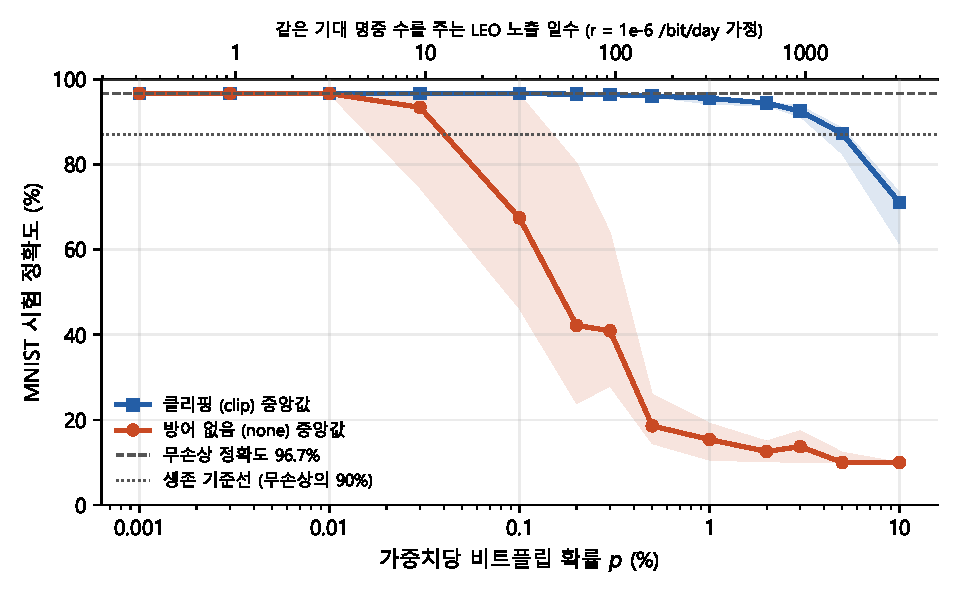
\includegraphics[width=0.95\linewidth]{fig_e1_dose_response}
  \caption{E1 용량--반응 곡선. 선은 10회 시행의 중앙값, 띠는 사분위범위(IQR)이다. 위쪽 축은 식~\eqref{eq:teq}로 환산한 LEO 노출 일수이다.}
  \label{fig:dose}
\end{figure}

\begin{table}[!htb]
  \centering\scriptsize
  \caption{E1 조건별 요약(각 10회). $\bar{k}$는 평균 명중 수, LEO 일수는 식~\eqref{eq:teq}($r=10^{-6}$/bit/day). 생존률은 정확도가 무손상의 90\,\% 이상인 시행의 비율, 붕괴율은 NaN/$\infty$가 발생한 시행의 비율.}
  \label{tab:e1}
  \begin{tabular}{rrr|rrrr|rrrr}
\toprule
$p$ (\%) & $\bar{k}$ & LEO 일수 & \multicolumn{4}{c|}{방어 없음} & \multicolumn{4}{c}{클리핑} \\
 & & & 중앙값 & IQR & 생존률 & 붕괴율 & 중앙값 & IQR & 생존률 & 붕괴율 \\
\midrule
0.001 & 1 & 0.3 & 96.7 & 96.7--96.7 & 1.0 & 0.0 & 96.7 & 96.7--96.7 & 1.0 & 0.0 \\
0.003 & 4 & 0.9 & 96.7 & 96.7--96.7 & 1.0 & 0.0 & 96.7 & 96.7--96.7 & 1.0 & 0.0 \\
0.01 & 12 & 3.1 & 96.6 & 96.6--96.7 & 1.0 & 0.0 & 96.7 & 96.7--96.7 & 1.0 & 0.0 \\
0.03 & 31 & 9.4 & 93.4 & 74.5--96.6 & 0.6 & 0.0 & 96.6 & 96.6--96.7 & 1.0 & 0.0 \\
0.1 & 104 & 31.3 & 67.4 & 46.2--96.5 & 0.4 & 0.0 & 96.6 & 96.5--96.7 & 1.0 & 0.0 \\
0.2 & 208 & 62.5 & 42.2 & 23.9--80.3 & 0.1 & 0.1 & 96.5 & 96.0--96.6 & 1.0 & 0.0 \\
0.3 & 308 & 93.8 & 40.9 & 27.9--64.0 & 0.0 & 0.0 & 96.4 & 96.3--96.6 & 1.0 & 0.0 \\
0.5 & 511 & 156.2 & 18.6 & 14.4--26.0 & 0.1 & 0.1 & 96.1 & 95.9--96.4 & 1.0 & 0.0 \\
1 & 1,019 & 312.5 & 15.4 & 10.6--19.2 & 0.0 & 0.2 & 95.5 & 94.1--95.9 & 0.9 & 0.0 \\
2 & 2,031 & 625.0 & 12.6 & 10.1--15.0 & 0.0 & 0.2 & 94.4 & 93.7--94.6 & 1.0 & 0.0 \\
3 & 3,060 & 937.5 & 13.7 & 10.1--17.5 & 0.0 & 0.2 & 92.5 & 91.2--93.8 & 0.9 & 0.0 \\
5 & 5,080 & 1,562.5 & 10.0 & 10.0--12.4 & 0.0 & 0.5 & 87.2 & 82.4--88.5 & 0.6 & 0.0 \\
10 & 10,178 & 3,125.0 & 10.0 & 10.0--10.0 & 0.0 & 0.9 & 71.0 & 61.4--73.5 & 0.0 & 0.0 \\
\bottomrule
\end{tabular}

\end{table}

\subsection{같은 선량, 다른 운명: 이봉 분포 (Q2)}
그림~\ref{fig:trials}는 시행 하나하나를 점으로 찍은 것이다. 방어 없음의 $p=0.03\,\%\sim0.3\,\%$ 구간에서는 같은 $p$라도 무손상에 가까운 시행(96\,\%대)과 크게 손상된 시행(\pThreeEmFourNoneMin{}\,\%까지)이 공존하며, 그 사이가 비어 있다. 예컨대 $p=0.1\,\%$의 10회 시행 중 4회는 96\,\% 이상, 나머지 6회는 33--78\,\%였다. 이 구간에서 명중 수 $k$는 시행 간에 거의 같으므로(표~\ref{tab:e1}의 $\bar{k}$ 참조), 차이는 명중 \emph{개수}가 아니라 어느 가중치의 어느 비트가 맞았는가에서 온다. 평균$\pm$표준편차로 요약하면 이 구조가 가려지며, 실제로 $p=0.03\,\%$의 평균은 80.1\,\%지만 중앙값은 \pThreeEmFourNoneMed{}\,\%이다.

\begin{figure}[!htb]
  \centering
  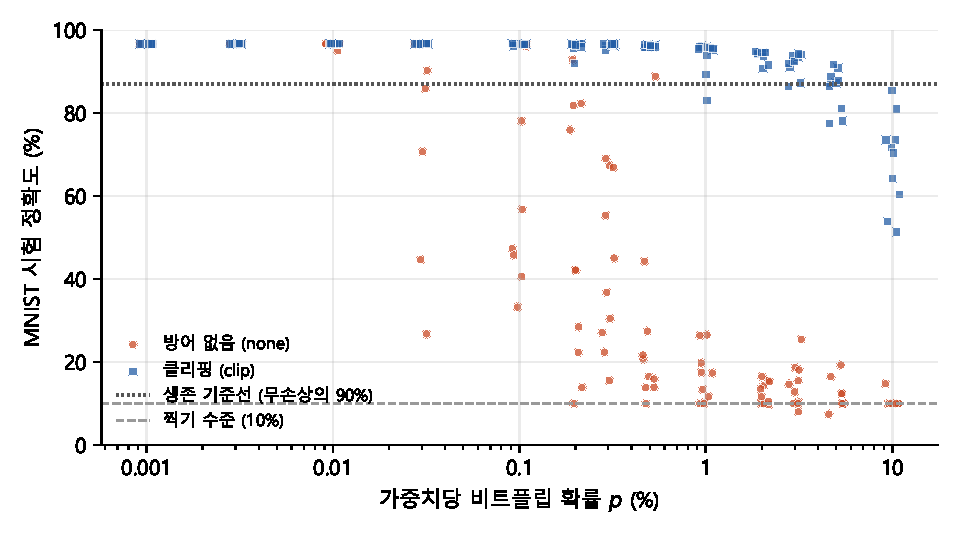
\includegraphics[width=0.95\linewidth]{fig_e1_trials}
  \caption{E1의 모든 시행(점 하나 = 시행 1회, 가로 위치는 겹침을 피하기 위해 약간 흔듦). 방어 없음은 중간 선량대에서 두 무리로 갈라진다.}
  \label{fig:trials}
\end{figure}

\subsection{붕괴(\texorpdfstring{NaN/$\infty$}{NaN/inf})의 출현}
붕괴는 방어 없음에서 $p=0.2\,\%$부터 나타나 $p=1\,\%$에서 \pOneEmTwoNoneCrash{}, $p=5\,\%$에서 \pFiveEmTwoNoneCrash{}, $p=10\,\%$에서 \pOneEmOneNoneCrash{}로 증가한다(그림~\ref{fig:survival}b). 전체 시행에서 명중 비트 중 지수부의 비율은 \ExpHitFrac{}\,\%, 부호 비트는 \SignHitFrac{}\,\%로 무작위 기대값(8/32, 1/32)과 일치한다. 그러나 붕괴와 큰 손상은 모두 지수부 명중, 특히 bit~30 명중이 $\pm\infty$ 또는 $10^{38}$ 크기의 가중치를 만들 때 발생한다(\ref{sec:prelim}절의 비트별 실험 참조). 클리핑 조건에서는 \NumTrials{}회 중 붕괴가 한 번도 없었다.

\begin{figure}[!htb]
  \centering
  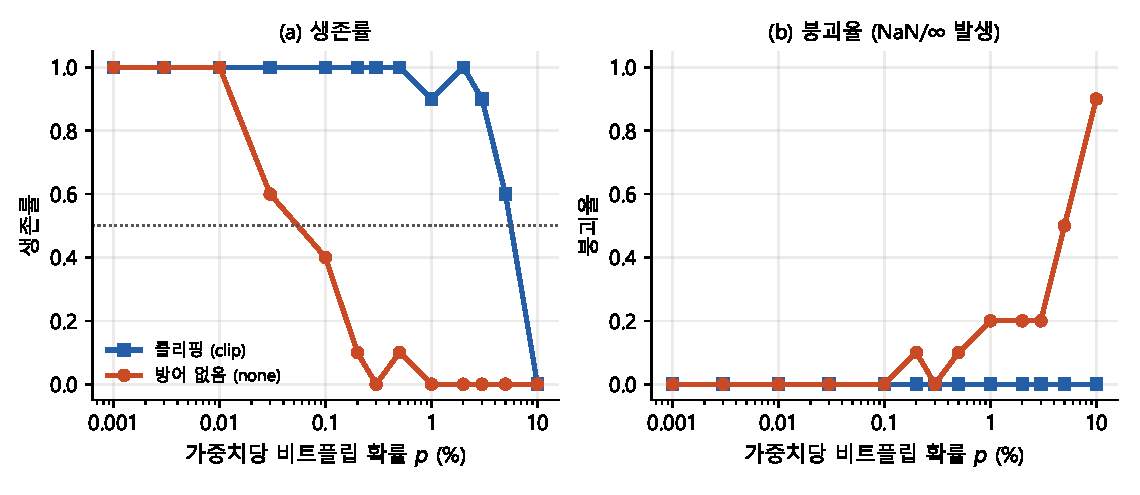
\includegraphics[width=0.95\linewidth]{fig_e1_survival_crash}
  \caption{(a) 생존률과 (b) 붕괴율. 점선은 생존률 50\,\%.}
  \label{fig:survival}
\end{figure}

\subsection{클리핑의 효과 (H3)}
클리핑은 생존률 1.0을 $p=0.5\,\%$까지 유지하고, $p=1\,\%$에서도 중앙값 \pOneEmTwoClipMed{}\,\%(방어 없음 \pOneEmTwoNoneMed{}\,\%), $p=5\,\%$에서 \pFiveEmTwoClipMed{}\,\%(방어 없음 \pFiveEmTwoNoneMed{}\,\%)를 기록하였다. 생존률이 50\,\%를 가로지르는 확률을 $\log p$ 선형 보간으로 구하면 방어 없음 $p_{50}\approx\PhalfNone\,\%$, 클리핑 $p_{50}\approx\PhalfClip\,\%$로, 클리핑은 견딜 수 있는 선량을 약 \PhalfRatio{}배 높였다. 클리핑도 $p=10\,\%$(가중치 열 개 중 하나가 손상)에서는 중앙값 \pOneEmOneClipMed{}\,\%로 떨어지는데, 이때의 손상은 $\infty$가 아니라 잘려서 $\pm3$이 된 수천 개의 가중치가 누적된 결과이다. 따라서 H3은 지지되며, 그 한계도 함께 드러났다.

\subsection{LEO 노출 일수로의 환산}
식~\eqref{eq:teq}에 따르면, $r=10^{-6}$/bit/day(Alsat-1 측정값~\citep{bentoutou2008}) 아래 이 모델은 하루에 약 \LeoFlipsPerDay{}개의 비트플립을 받는다. JASON-2 측정값($4.8\times10^{-7}$)을 쓰면 일수는 약 2배로 늘어난다. 생존률 50\,\%에 해당하는 선량은 방어 없음에서 약 \PhalfNoneDays{}일, 클리핑에서 약 \PhalfClipDays{}일이다. 즉 방어 없는 float32 신경망은 수 주 안에 절반의 확률로 10\,\% 이상의 성능 손실을 겪지만, 가장 단순한 클리핑만으로도 수 년 규모로 늘어난다. 이 수치는 $r$에 정비례하므로, 궤도·태양 활동·소자에 따라 $r$이 10배 달라지면 일수도 10배 달라진다.

\subsection{모델 크기 축 (E1-M): 생존을 결정하는 것은 확률이 아니라 명중 수}
\label{sec:models}
같은 실험을 표~\ref{tab:model}의 세 모델에 반복하였다($p$ 9단계, 큰 모델은 $10^{-6}$부터, 각 10회). 그림~\ref{fig:models}(a)(c)에서 보듯 $p$를 가로축으로 두면 큰 모델일수록 곡선이 왼쪽으로 이동한다. 방어 없음의 생존률 50\,\% 지점은 \code{mnist\_linear} $p_{50}=\PhalfNoneLinear\,\%$에서 \code{resnet18\_t10} $p_{50}=\PhalfNoneResnet\,\%$로 약 50배 낮아진다. 그러나 가로축을 평균 명중 수 $\bar{k}=pN_w$로 바꾸면(그림~\ref{fig:models_hits}) 네 모델의 생존률 곡선이 거의 한 곡선으로 겹친다. 생존률 50\,\%에 해당하는 명중 수 $k_{50}$은 \KhalfNoneLinear{}, \KhalfNoneCnn{}, \KhalfNoneCifar{}, \KhalfNoneResnet{}개로, 가중치 수가 110배 차이 나는 모델 사이에서 2배 안에 든다(표~\ref{tab:models}). 즉 방어 없는 float32 모델의 생존은 ``몇 개의 비트가 뒤집혔는가''로 결정되며, 수십 개의 무작위 명중 가운데 지수 최상위 비트의 $0\to1$ 플립이 하나라도 섞이면 무너진다는 \ref{sec:prelim}절의 설명과 맞는다.

\begin{figure}[!htb]
  \centering
  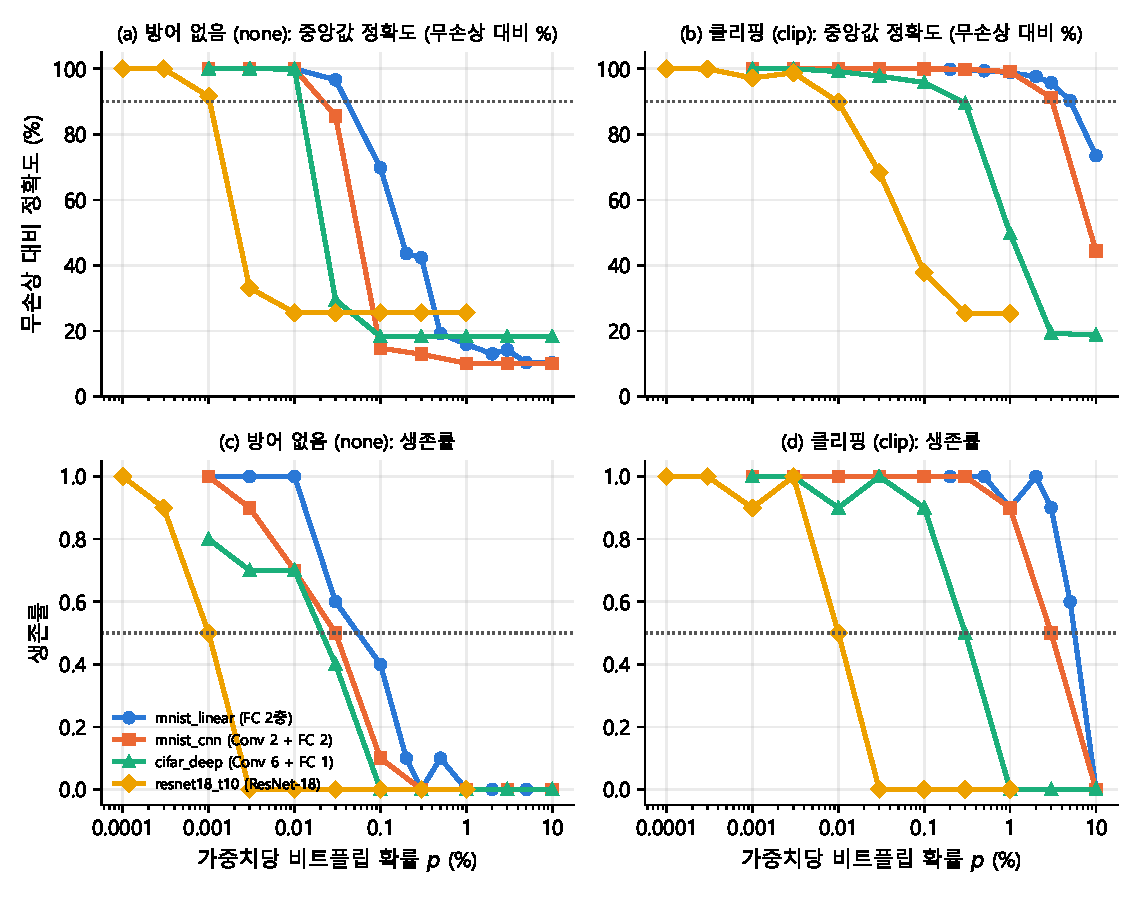
\includegraphics[width=0.95\linewidth]{fig_e1_models}
  \caption{E1-M: 네 모델의 용량--반응. (a)(b) 무손상 대비 중앙값 정확도, (c)(d) 생존률. 왼쪽 열은 방어 없음, 오른쪽 열은 클리핑.}
  \label{fig:models}
\end{figure}

\begin{figure}[!htb]
  \centering
  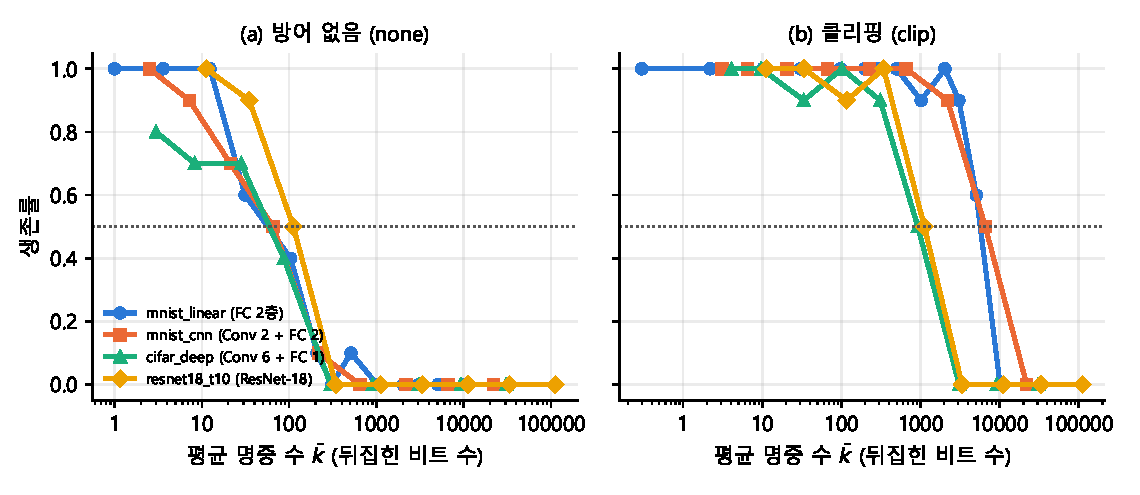
\includegraphics[width=0.95\linewidth]{fig_e1_models_hits}
  \caption{가로축을 평균 명중 수 $\bar{k}$로 바꾼 생존률. 방어 없음(a)에서는 네 모델이 한 곡선으로 모인다.}
  \label{fig:models_hits}
\end{figure}

\begin{table}[!htb]
  \centering\scriptsize
  \caption{E1-M 모델별 요약. 명중/일은 $rN_{\mathrm{bits}}$($r=10^{-6}$/bit/day), $p_{50}$·$k_{50}$은 생존률이 50\,\%를 가로지르는 확률과 그때의 기대 명중 수($\log p$ 선형 보간), LEO 일수는 식~\eqref{eq:teq}.}
  \label{tab:models}
  \begin{tabular}{lrrrr|rrr|rr}
\toprule
모델 & $N_w$ & $N_{\mathrm{bits}}$ & 무손상 & 명중/일 & \multicolumn{3}{c|}{방어 없음, 생존률 50\%} & \multicolumn{2}{c}{클리핑, 생존률 50\%} \\
 & & & 정확도 & ($r$=$10^{-6}$) & $p_{50}$ (\%) & $k_{50}$ & LEO 일수 & $p_{50}$ (\%) & LEO 일수 \\
\midrule
\code{mnist\_linear} & 101,632 & 3,252,224 & 96.7 & 3.3 & 0.0548 & 56 & 17일 & 5.6 & 1,754일 \\
\code{mnist\_cnn} & 220,064 & 7,042,048 & 98.7 & 7.0 & 0.03 & 66 & 9일 & 3 & 937일 \\
\code{cifar\_deep} & 307,040 & 9,825,280 & 54.6 & 9.8 & 0.0208 & 64 & 7일 & 0.3 & 94일 \\
\code{resnet18\_t10} & 11,172,032 & 357,505,024 & 39.1 & 357.5 & 0.001 & 112 & 7.5시간 & 0.01 & 3일 \\
\bottomrule
\end{tabular}

\end{table}

이 결과는 LEO 노출 시간의 해석을 바꾼다. 하루 명중 수는 $rN_{\mathrm{bits}}$로 모델 크기에 비례하므로, 생존률 50\,\%까지의 시간은 $T_{50}\approx k_{50}/(rN_{\mathrm{bits}})$, 즉 모델 크기에 반비례한다. 표~\ref{tab:models}에서 방어 없음의 $T_{50}$은 \code{mnist\_linear}의 \DaysNoneLinear{}에서 \code{resnet18\_t10}의 \DaysNoneResnet{}으로 줄어든다. $k_{50}\approx60$--$110$을 그대로 적용하면 ResNet-50(2{,}560만 파라미터)은 \TfiftyResnetFifty{}, 1억 파라미터급 모델은 \TfiftyHundredMMin{} 안팎이다(\ref{sec:fit}절의 모형으로 계산). 방어 없는 float32 탑재 신경망은 궤도에서 하루를 버티지 못한다는 뜻이다.

클리핑의 이득은 과제의 여유에 따라 달랐다. $p_{50}$의 비(클리핑/방어 없음)는 MNIST 두 모델에서 약 \ClipGainLinear{}배와 \ClipGainCnn{}배였으나, 무손상 정확도가 낮은 CIFAR-10 두 모델에서는 \ClipGainCifar{}배와 \ClipGainResnet{}배에 그쳤다. 클리핑은 $\infty$/NaN 붕괴는 완전히 막지만(네 모델 모두 클리핑 조건에서 붕괴 0), $\pm3$으로 잘린 수백 개의 가중치가 남기는 누적 손상은 막지 못하며, 클래스 간 여유가 작은 모델은 그 손상에 더 민감하다. 그림~\ref{fig:models_hits}(b)에서 클리핑 조건의 곡선은 방어 없음과 달리 모델별로 갈라지는데, 이것이 그 증거다.

\subsection{궤도 모드 (E3): SAA에 몰려 들어오는 명중}
\label{sec:e3}
\code{leo\_saa} 모드에서는 하루 명중의 90\,\%가 세 번의 SAA 통과(각 12분)에 몰려 들어온다. 표~\ref{tab:e3}와 그림~\ref{fig:e3}에서 보듯 결과는 stress 모드와 같은 명중 수에서 같은 생존률을 보였다. 방어 없는 \code{mnist\_linear}는 7일까지 생존률 0.9--1.0을 유지하다가 30일에 0.3, 90일에 0.1로 떨어졌고, \code{mnist\_cnn}은 14일에 0.3, 60일에 0이었다. 클리핑은 90일(명중 약 300--630개)까지 생존률 1.0이었다. 추론 시점에 명중이 시간적으로 몰려 있는지 여부는 결과에 영향을 주지 않았는데, 이는 추론 중 가중치가 갱신되지 않아 명중의 \emph{순서}가 무의미하기 때문이다. 학습 중 주입(E4)에서는 다를 수 있다.

\begin{figure}[!htb]
  \centering
  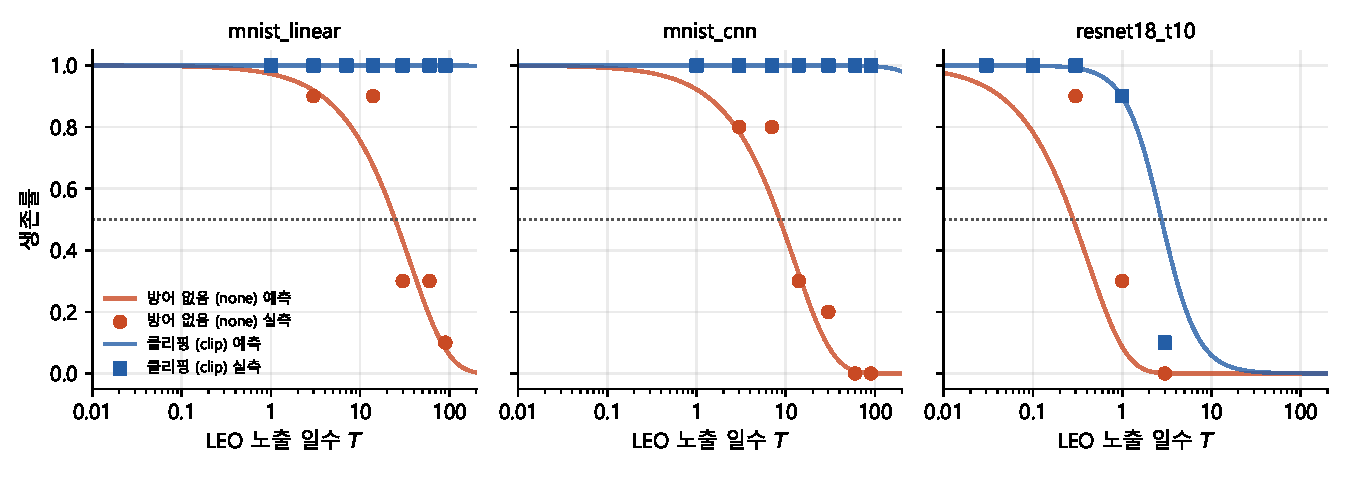
\includegraphics[width=0.95\linewidth]{fig_e3_leo}
  \caption{E3: 궤도 모드(\code{leo\_saa}) 실측 생존률(점)과 stress 모드로 맞춘 수학 모델의 예측(선). 모델은 E3 데이터를 보지 않았다.}
  \label{fig:e3}
\end{figure}

\begin{table}[!htb]
  \centering\scriptsize
  \caption{E3 궤도 모드 실측 생존률과 모델 예측(식~\eqref{eq:modelA}, \eqref{eq:modelB}, stress 데이터로만 맞춤). 예측은 각 조건에 실제로 전달된 평균 명중 수 $\bar{k}$를 넣어 계산하였다. 전체 \EthreeN{}개 조건에서 평균 절대 오차 \EthreeMAE{}, 최대 \EthreeMaxErr{}.}
  \label{tab:e3}
  \begin{tabular}{lr|rrr|rrr}
\toprule
모델 & $T$ (일) & \multicolumn{3}{c|}{방어 없음} & \multicolumn{3}{c}{클리핑} \\
 & & $\bar{k}$ & 실측 & 예측 & $\bar{k}$ & 실측 & 예측 \\
\midrule
\code{mnist\_linear} & 1 & 4 & 1.0 & 0.97 & 4 & 1.0 & 1.00 \\
\code{mnist\_linear} & 3 & 10 & 0.9 & 0.92 & 11 & 1.0 & 1.00 \\
\code{mnist\_linear} & 7 & 23 & 1.0 & 0.82 & 24 & 1.0 & 1.00 \\
\code{mnist\_linear} & 14 & 48 & 0.9 & 0.66 & 51 & 1.0 & 1.00 \\
\code{mnist\_linear} & 30 & 98 & 0.3 & 0.43 & 98 & 1.0 & 1.00 \\
\code{mnist\_linear} & 60 & 195 & 0.3 & 0.18 & 200 & 1.0 & 1.00 \\
\code{mnist\_linear} & 90 & 287 & 0.1 & 0.08 & 298 & 1.0 & 1.00 \\
\code{mnist\_cnn} & 1 & 7 & 1.0 & 0.92 & 6 & 1.0 & 1.00 \\
\code{mnist\_cnn} & 3 & 20 & 0.8 & 0.79 & 18 & 1.0 & 1.00 \\
\code{mnist\_cnn} & 7 & 48 & 0.8 & 0.58 & 46 & 1.0 & 1.00 \\
\code{mnist\_cnn} & 14 & 100 & 0.3 & 0.32 & 98 & 1.0 & 1.00 \\
\code{mnist\_cnn} & 30 & 217 & 0.2 & 0.08 & 210 & 1.0 & 1.00 \\
\code{mnist\_cnn} & 60 & 439 & 0.0 & 0.01 & 413 & 1.0 & 1.00 \\
\code{mnist\_cnn} & 90 & 646 & 0.0 & 0.00 & 632 & 1.0 & 1.00 \\
\code{resnet18\_t10} & 0.03 & 1 & 1.0 & 0.99 & 1 & 1.0 & 1.00 \\
\code{resnet18\_t10} & 0.1 & 3 & 1.0 & 0.98 & 57 & 1.0 & 1.00 \\
\code{resnet18\_t10} & 0.3 & 95 & 0.9 & 0.52 & 102 & 1.0 & 0.99 \\
\code{resnet18\_t10} & 1 & 364 & 0.3 & 0.08 & 354 & 0.9 & 0.90 \\
\code{resnet18\_t10} & 3 & 1,072 & 0.0 & 0.00 & 1,054 & 0.1 & 0.46 \\
\bottomrule
\end{tabular}

\end{table}

\subsection{방어 비교 (E5): 무엇이 얼마나 늘려 주는가}
\label{sec:e5}
그림~\ref{fig:e5}와 표~\ref{tab:e5}는 \code{mnist\_linear}에서 방어 6종을 비교한 것이다. 패리티와 TMR은 실험한 최대 선량($p=3\,\%$, 명중 약 3{,}000개)까지 생존률 1.0, 중앙값 정확도 96.3\,\% 이상이었다. 패리티는 1비트 오류를 전부 검출해 해당 가중치를 0으로 되돌리므로 손상이 ``가중치 3\,\%를 0으로 만든 것''에 그치고, TMR은 같은 가중치가 세 복제본 중 둘 이상에서 맞을 때만 손상되므로 $k\ll N_w$에서는 사실상 무손상이다. 클리핑의 이득은 모델 B로 맞춘 $k_{50}$의 비로 약 \GainEClip{}배였다(표~\ref{tab:e1}의 보간값 \PhalfRatio{}배와 같은 자릿수). 로짓 중앙값 앙상블은 $p=0.1\,\%$까지 생존률 0.8을 유지했지만 $0.3\,\%$에서 0으로 떨어져 이득이 \GainEEnsMed{}배에 그쳤고, 로짓 평균 앙상블은 이득 \GainEEns{}배로 방어 없음보다 \emph{나빴다}. 평균은 복제본 다섯 개 중 하나라도 $10^{38}$ 크기의 로짓을 내면 그에 지배되는데, 복제본이 다섯이므로 그런 복제본이 생길 확률도 다섯 배이기 때문이다. 중앙값이 평균보다 이상치에 강하다는 통계의 기본 사실이 방어 설계에서 그대로 드러난다. 3.5절의 예측 $G=1/5=0.2$보다 실측 이득(\GainEEns{})이 큰 것은, 손상된 복제본 하나의 피해가 정상 복제본 넷의 평균에 일부 희석되기 때문이다.

패리티와 TMR의 한계를 보기 위해 $p$를 50\,\%까지 올린 결과가 표~\ref{tab:e5high}이다. TMR은 $p=10\,\%$에서 생존률 0.8, $20\,\%$에서 0으로 무너졌다. 식~\eqref{eq:tmr}에 \code{mnist\_linear}의 $q$를 넣으면 $k_{50}^{\mathrm{TMR}}\approx\KfiftyTmrPred$(즉 $p\approx\PfiftyTmrPred\,\%$)로, 모델 B로 실측에 맞춘 $k_{50}$(표~\ref{tab:e5}의 10{,}639)과 15\,\% 안에서 맞는다. 즉 TMR의 이득은 이득 상수가 아니라 $\sqrt{N_w/q}$에 비례하는 양이며, 가중치가 많은 모델일수록 TMR이 상대적으로 더 유리하다. 패리티는 가중치의 20\,\%가 0이 되어도 생존률 1.0, 30\,\%에서 0.8(중앙값 88.3\,\%)로, 가장 강건한 동시에 가장 싼 방어였다(메모리 +1/32).

\begin{table}[!htb]
  \centering\scriptsize
  \caption{고선량에서의 TMR과 패리티(\code{mnist\_linear}, 각 10회). TMR 예측은 식~\eqref{eq:tmr}의 $\exp(-3k^2q/(32N_w))$.}
  \label{tab:e5high}
  \begin{tabular}{lrr|rr|rr}
\toprule
$p$ (\%) & $\bar{k}$ & $k/N_w$ & TMR 실측 & TMR 예측 & 패리티 실측 & 패리티 중앙값 \\
\midrule
0.03 & 30 & 0.00 & 1.0 & 1.00 & 1.0 & 96.7 \\
0.1 & 102 & 0.00 & 1.0 & 1.00 & 1.0 & 96.7 \\
0.3 & 306 & 0.00 & 1.0 & 1.00 & 1.0 & 96.6 \\
1 & 1,021 & 0.01 & 1.0 & 0.99 & 1.0 & 96.6 \\
3 & 3,061 & 0.03 & 1.0 & 0.93 & 1.0 & 96.3 \\
5 & 5,108 & 0.05 & 1.0 & 0.81 & 1.0 & 96.1 \\
10 & 10,188 & 0.10 & 0.8 & 0.44 & 1.0 & 95.3 \\
20 & 20,331 & 0.20 & 0.0 & 0.04 & 1.0 & 92.3 \\
30 & 30,501 & 0.30 & 0.0 & 0.00 & 0.8 & 88.3 \\
50 & 50,842 & 0.50 & 0.0 & 0.00 & 0.0 & 74.2 \\
\bottomrule
\end{tabular}

\end{table}

\begin{figure}[!htb]
  \centering
  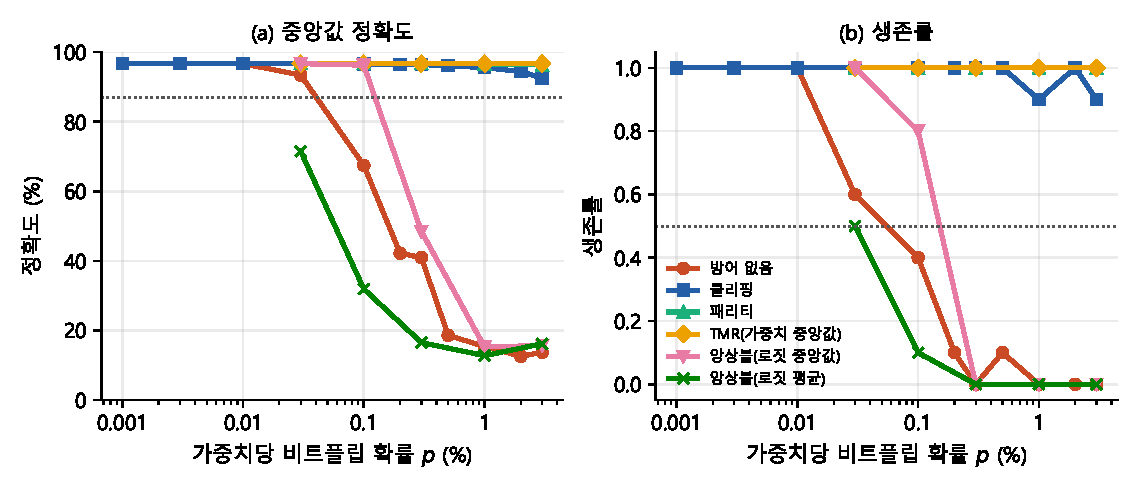
\includegraphics[width=0.95\linewidth]{fig_e5_defenses}
  \caption{E5: \code{mnist\_linear}의 방어 6종. (a) 중앙값 정확도, (b) 생존률. 패리티와 TMR은 겹쳐서 TMR 아래에 있다.}
  \label{fig:e5}
\end{figure}

\begin{table}[!htb]
  \centering\scriptsize
  \caption{E5 방어별 중앙값 정확도(괄호는 생존률)와 모델 B로 맞춘 $k_{50}$, 이득 $G_d$. ``$>$''는 실험 범위 안에서 생존률이 50\,\% 아래로 내려가지 않았음을 뜻한다.}
  \label{tab:e5}
  \setlength{\tabcolsep}{3pt}
\begin{tabular}{lrrrrr|rr}
\toprule
방어 & $p$=0.03\% & $p$=0.1\% & $p$=0.3\% & $p$=1\% & $p$=3\% & $k_{50}$ & 이득 \\
\midrule
없음 & 93.4 (0.6) & 67.4 (0.4) & 40.9 (0.0) & 15.4 (0.0) & 13.7 (0.0) & 62 & 1.0 \\
클리핑 & 96.6 (1.0) & 96.6 (1.0) & 96.4 (1.0) & 95.5 (0.9) & 92.5 (0.9) & 5,155 & 83.8 \\
패리티 & 96.7 (1.0) & 96.7 (1.0) & 96.6 (1.0) & 96.6 (1.0) & 96.3 (1.0) & 31,371 & 509.7 \\
TMR & 96.7 (1.0) & 96.7 (1.0) & 96.7 (1.0) & 96.7 (1.0) & 96.7 (1.0) & 10,639 & 172.8 \\
앙상블(중앙값) & 96.7 (1.0) & 96.2 (0.8) & 48.5 (0.0) & 15.3 (0.0) & 15.7 (0.0) & 109 & 1.8 \\
앙상블(평균) & 71.5 (0.5) & 31.9 (0.1) & 16.5 (0.0) & 12.8 (0.0) & 16.2 (0.0) & 30 & 0.5 \\
\bottomrule
\end{tabular}

\end{table}

\subsection{비트별 치명도 (E2): 32비트 중 하나만 위험하다}
\label{sec:prelim}
정확히 한 비트만 한 번 뒤집는 실험(E2)으로 식~\eqref{eq:q}의 분해를 직접 검증하였다. 부호 비트(31), 지수 비트 8개(30--23), 가수 비트 4개(22, 16, 10, 0)를 각각 \code{mnist\_linear}는 50회, 나머지 세 모델은 30회 뒤집었다. 그림~\ref{fig:e2}와 표~\ref{tab:e2}의 결과는 단순하다. \textbf{bit~30을 제외한 모든 비트에서 생존률은 1.00이었다.} 부호 반전은 가중치 하나의 부호를 바꿀 뿐이고, bit~29--23은 학습된 가중치($|w|<1$, $E\le126$)에서 대부분 이미 1이어서 $1\to0$ 플립이 값을 \emph{줄이며}, 0인 비트(bit~25, 23 등)가 $0\to1$로 바뀌어도 값은 2--16배 커지는 데 그쳐 수만 개 가중치의 합에 묻힌다. 오직 bit~30의 $0\to1$ 플립만이 $2^{128}$배라는 규모로 가중치 하나를 네트워크 전체 위에 올려놓는다.

bit~30 단일 명중의 생존률은 \code{mnist\_linear} \SthirtyEtwoLinear{} \SthirtyCILinear{}, \code{mnist\_cnn} \SthirtyEtwoCnn{} \SthirtyCICnn{}, \code{cifar\_deep} \SthirtyEtwoCifar{} \SthirtyCICifar{}, \code{resnet18\_t10} \SthirtyEtwoResnet{} \SthirtyCIResnet{}였다. 모델 A에서 bit~30 명중 하나의 생존률은 $1-\pi_+\alpha = 1-32q$이므로, E1로 맞춘 $q$가 예측하는 값은 각각 \SthirtyPredLinear{}, \SthirtyPredCnn{}, \SthirtyPredCifar{}, \SthirtyPredResnet{}이다. 네 모델 모두 예측이 신뢰구간 안에 들었다. 거꾸로 E2에서 독립적으로 $q_{E2}=\frac{1}{32}\sum_b(1-S_b)$를 구하면 \QEtwoLinear{}, \QEtwoCnn{}, \QEtwoCifar{}, \QEtwoResnet{}으로 E1 적합값(\QLinear{}, \QCnn{}, \QCifar{}, \QResnet{})과 맞는다. 즉 수십 개의 무작위 명중에서 본 붕괴율과 단 한 비트의 치명도는 같은 수 $q$로 연결되며, 그 수는 ``bit~30이 뽑힐 확률 $1/32$ $\times$ 양수 가중치 $\times$ 활성 경로''로 설명된다. 클리핑 조건에서는 bit~30을 포함한 모든 비트에서 생존률 1.00이었다. 뒤집힌 가중치 하나가 $\pm3$으로 잘리는 것은 무해하기 때문이다.

\begin{figure}[!htb]
  \centering
  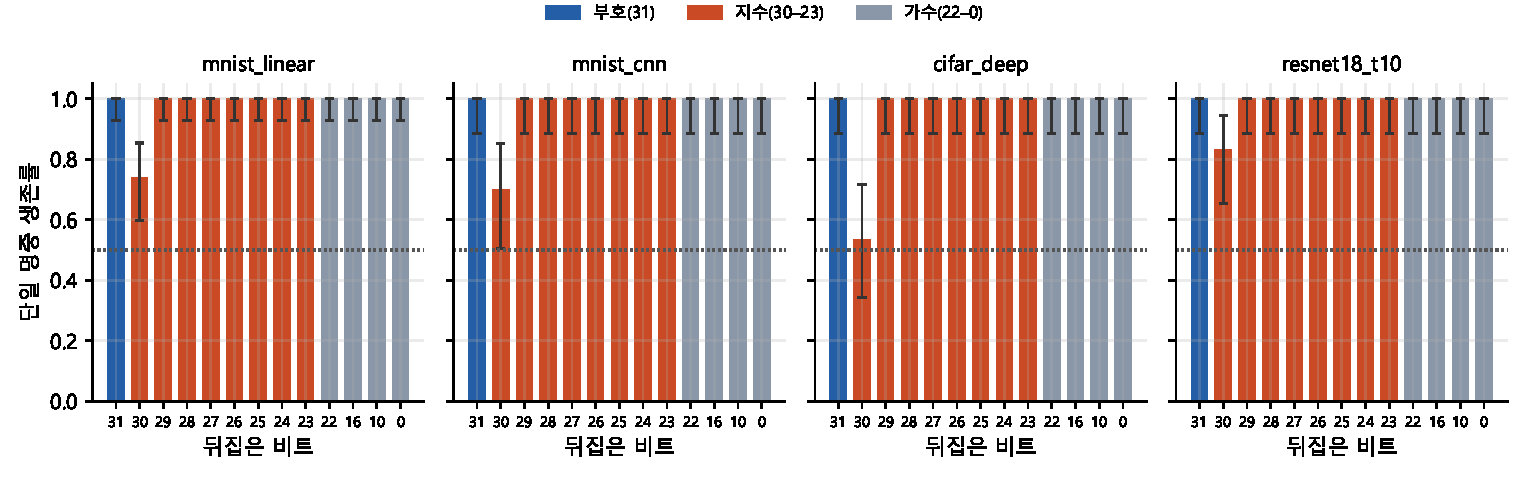
\includegraphics[width=0.95\linewidth]{fig_e2_bits}
  \caption{E2 비트 지도: 비트 하나를 정확히 한 번 뒤집었을 때의 생존률(방어 없음)과 Clopper--Pearson 95\,\% 신뢰구간. 32비트 가운데 bit~30만 치명적이다.}
  \label{fig:e2}
\end{figure}

\begin{table}[!htb]
  \centering\scriptsize
  \caption{E2 비트별 단일 명중 생존률 [95\,\% 신뢰구간]. 아래 세 줄은 E2에서 독립 추정한 $q_{E2}$, E1 적합 $q$, 그리고 bit~30 생존률의 예측($1-32q$)과 실측.}
  \label{tab:e2}
  \setlength{\tabcolsep}{4pt}
\begin{tabular}{lccccc}
\toprule
비트 & \code{mnist\_linear} & \code{mnist\_cnn} & \code{cifar\_deep} & \code{resnet18\_t10} & \code{mnist\_linear} 클리핑 \\
\midrule
31 (부호) & 1.00 [0.93, 1.00] & 1.00 [0.88, 1.00] & 1.00 [0.88, 1.00] & 1.00 [0.88, 1.00] & 1.00 \\
30 (지수 MSB) & 0.74 [0.60, 0.85] & 0.70 [0.51, 0.85] & 0.53 [0.34, 0.72] & 0.83 [0.65, 0.94] & 1.00 \\
29 (지수) & 1.00 [0.93, 1.00] & 1.00 [0.88, 1.00] & 1.00 [0.88, 1.00] & 1.00 [0.88, 1.00] & 1.00 \\
28 (지수) & 1.00 [0.93, 1.00] & 1.00 [0.88, 1.00] & 1.00 [0.88, 1.00] & 1.00 [0.88, 1.00] & 1.00 \\
27 (지수) & 1.00 [0.93, 1.00] & 1.00 [0.88, 1.00] & 1.00 [0.88, 1.00] & 1.00 [0.88, 1.00] & 1.00 \\
26 (지수) & 1.00 [0.93, 1.00] & 1.00 [0.88, 1.00] & 1.00 [0.88, 1.00] & 1.00 [0.88, 1.00] & 1.00 \\
25 (지수) & 1.00 [0.93, 1.00] & 1.00 [0.88, 1.00] & 1.00 [0.88, 1.00] & 1.00 [0.88, 1.00] & 1.00 \\
24 (지수) & 1.00 [0.93, 1.00] & 1.00 [0.88, 1.00] & 1.00 [0.88, 1.00] & 1.00 [0.88, 1.00] & 1.00 \\
23 (지수) & 1.00 [0.93, 1.00] & 1.00 [0.88, 1.00] & 1.00 [0.88, 1.00] & 1.00 [0.88, 1.00] & 1.00 \\
22 (가수) & 1.00 [0.93, 1.00] & 1.00 [0.88, 1.00] & 1.00 [0.88, 1.00] & 1.00 [0.88, 1.00] & 1.00 \\
16 (가수) & 1.00 [0.93, 1.00] & 1.00 [0.88, 1.00] & 1.00 [0.88, 1.00] & 1.00 [0.88, 1.00] & 1.00 \\
10 (가수) & 1.00 [0.93, 1.00] & 1.00 [0.88, 1.00] & 1.00 [0.88, 1.00] & 1.00 [0.88, 1.00] & 1.00 \\
0 (가수) & 1.00 [0.93, 1.00] & 1.00 [0.88, 1.00] & 1.00 [0.88, 1.00] & 1.00 [0.88, 1.00] & 1.00 \\
\midrule
$q_{E2}=\frac{1}{32}\sum_b(1-S_b)$ & 0.0081 & 0.0094 & 0.0146 & 0.0052 &  \\
$q$ (E1 적합) & 0.0086 & 0.0115 & 0.0163 & 0.0068 &  \\
bit 30 예측 $1-32q$ / 실측 & 0.72 / 0.74 & 0.63 / 0.70 & 0.48 / 0.53 & 0.78 / 0.83 &  \\
\bottomrule
\end{tabular}

\end{table}

\subsection{수학적 모델의 적합과 예측}
\label{sec:fit}
표~\ref{tab:fit}과 그림~\ref{fig:fit}에 두 모형의 적합 결과를 정리하였다. 모델 A의 치명 확률 $q$는 네 모델에서 \QMin{}--\QMax{}(중앙값 \QMedian{})로, 가중치 수가 110배 다른 모델 사이에서 2.4배 안에 들었다(H4 지지). 식~\eqref{eq:q}로 분해한 유효 전파 비율 $\alpha$는 \AlphaMin{}--\AlphaMax{}였다. MNIST 모델의 $\alpha\approx0.5$--$0.8$은 ``입력의 15\,\%는 항상 0인 픽셀이고 각 픽셀이 평균 19\,\%의 이미지에서만 0이 아니다''라는 사실과 맞으며, CIFAR-10처럼 모든 픽셀이 값을 갖는 입력에서는 $\alpha$가 1에 가깝다. 즉 $q$는 ``$1/32$에 양수 비율과 입력의 밀도를 곱한 값''으로 거의 예측된다. 모델 A의 생존률 예측 오차(평균 절대 오차)는 stress 데이터에서 0.02--0.06이었다. ``네 모델의 $q$가 같다''는 귀무가설을 가능도비로 검정하면 $D=\LrtD$, 자유도 \LrtDf{}, $p=\LrtP$로 5\,\% 수준에서 기각되지 않으며, 공통 $q=\QCommon$이다. 즉 데이터는 ``치명 확률은 모델 크기와 구조에 무관하다''(H4)와 양립한다.

\begin{figure}[!htb]
  \centering
  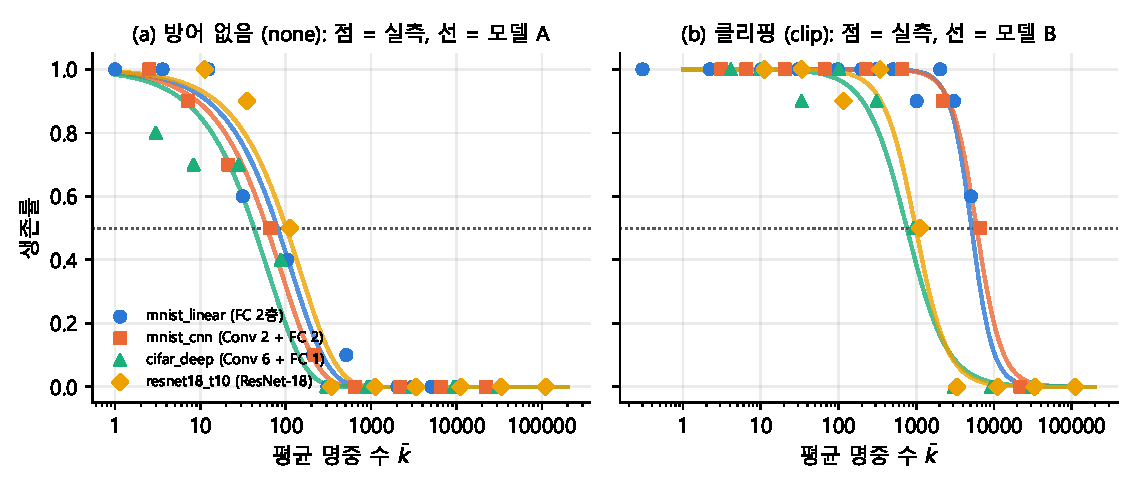
\includegraphics[width=0.95\linewidth]{fig_model_fit}
  \caption{실측 생존률(점)과 적합된 모델. (a) 방어 없음은 모델 A($e^{-qk}$), (b) 클리핑은 모델 B(로그-로지스틱).}
  \label{fig:fit}
\end{figure}

\begin{table}[!htb]
  \centering\scriptsize
  \caption{적합된 파라미터. $k_{50}^{A}=\ln2/q$, MAE는 stress 데이터에서의 생존률 평균 절대 오차, $T_{50}$ 예측은 $r=10^{-6}$/bit/day.}
  \label{tab:fit}
  \begin{tabular}{llrrrr|rrr|r}
\toprule
모델 & 방어 & $\pi_+$ & $q$ & $\alpha$ & $k_{50}^{A}$ & $k_{50}^{B}$ & $\beta$ & MAE & $T_{50}$ 예측 \\
\midrule
\code{mnist\_linear} & 없음 & 0.49 & 0.0086 & 0.56 & 80 & 62 & 1.7 & 0.04 & 25일 \\
 & 클리핑 & & & & & 5,155 & 3.2 & 0.03 & 1,585일 \\
\code{mnist\_cnn} & 없음 & 0.47 & 0.0115 & 0.78 & 60 & 48 & 1.4 & 0.02 & 9일 \\
 & 클리핑 & & & & & 5,994 & 2.7 & 0.01 & 851일 \\
\code{cifar\_deep} & 없음 & 0.42 & 0.0163 & 1.24 & 42 & 30 & 1.0 & 0.06 & 4일 \\
 & 클리핑 & & & & & 758 & 1.7 & 0.04 & 77일 \\
\code{resnet18\_t10} & 없음 & 0.46 & 0.0068 & 0.48 & 101 & 99 & 2.7 & 0.04 & 6.8시간 \\
 & 클리핑 & & & & & 985 & 2.1 & 0.04 & 3일 \\
\bottomrule
\end{tabular}

\end{table}

가장 중요한 검증은 E3이다. stress 데이터로만 맞춘 모델 A·B로 궤도 모드의 생존률을 예측하면, \EthreeN{}개 조건에서 평균 절대 오차 \EthreeMAE{}, 최대 \EthreeMaxErr{}이었다(표~\ref{tab:e3}). 가장 큰 오차는 \code{resnet18\_t10}의 $T=0.3$일 방어 없음(예측 0.52, 실측 0.9)과 $T=3$일 클리핑(예측 0.46, 실측 0.1)으로, 둘 다 생존률이 50\,\% 부근을 지나는 가장 가파른 구간이라 10회 시행의 이항 잡음($\pm0.3$)이 가장 큰 곳이다. 명중이 시간적으로 몰려 들어와도 식~\eqref{eq:modelA}이 그대로 맞는다.

이제 이 모형으로 임의의 조합을 계산할 수 있다. 네 모델의 중앙값 $q=\QMedian$을 쓰면 ResNet-50(2{,}560만 파라미터)이 방어 없이 LEO에서 생존률 50\,\%에 이르는 시간은 \TfiftyResnetFifty{}, 1억 파라미터 모델은 \TfiftyHundredMMin{}이다. 클리핑을 켜면 여유가 큰 과제에서 약 100배(수 년), 여유가 작은 과제에서 10--15배(수 일)로 늘어나고, 패리티나 TMR을 쓰면 실험 범위 안에서는 한계를 찾지 못했다. 반대로 요구 생존률 $S^\ast$와 임무 기간 $T$가 주어지면 허용 가능한 모델 크기 $N_{\mathrm{bits}}\le-\ln S^\ast/(q\,r\,T)$를 바로 구할 수 있다.

\todo{E4(학습 중 주입)는 \code{src/seu\_suite\_colab.ipynb}의 3-5절 셀로 실행할 수 있으나 결과 CSV가 아직 저장소에 없다. 학습 중에는 명중의 시간 순서가 의미를 가지므로, E3와 달리 SAA 집중 효과를 볼 수 있는 유일한 실험이다.}

% ------------------------------------------------------------
\section{논의}

\subsection{왜 ``개수''가 아니라 ``위치''인가}
식~\eqref{eq:float32}에서 가수 비트는 값을 최대 2배 이내로만 바꾸지만 지수 비트는 $2^{2^{j}}$배로 바꾼다. 신경망은 수천 개의 가중치가 합쳐지는 구조라 가수 비트 수십 개의 오류는 통계적으로 상쇄되지만, 지수 최상위 비트 하나는 $10^{38}$ 크기의 항을 만들어 합 전체를 지배한다. 이 항은 다음 층과의 곱셈에서 다시 증폭되어(2.2절의 $\delta\cdot a^{n}$) 출력층 전체를 오염시킨다. 중학교 수학으로 말하면, 평균은 이상치 하나에 끌려가지만 중앙값은 그렇지 않다는 사실이 TMR(중앙값)이 평균 앙상블보다 강건한 이유와 정확히 같다.

\subsection{이봉 분포와 요약 통계의 선택}
중간 선량대에서 결과가 두 무리로 갈라지는 현상은 ``위험한 비트가 맞았는가''라는 베르누이 사건이 결과를 지배하기 때문이다. 명중 $k$개 중 bit~30 명중이 하나도 없을 확률은 $(31/32)^{k}$이며, $k=31$이면 약 37\,\%, $k=104$이면 약 4\,\%이다. 그러나 bit~30 명중이 있어도 해당 가중치의 지수 비트가 이미 1이었다면($|w|\ge2$) 오히려 값이 작아져 피해가 없으므로, 실제 생존률은 이보다 높다. 이 구조에서는 평균이 ``아무도 겪지 않은'' 중간값을 보고하게 되므로, 신경망 내결함성 보고에서는 중앙값과 생존률을 함께 제시해야 한다.

\subsection{선행 연구와의 비교}
\label{sec:related}
표~\ref{tab:related}에 본 연구와 비교 가능한 선행 연구의 수치를 모았다. 비트당 오류율(BER)로 보고된 결과와 비교할 때는 본 연구의 가중치당 확률 $p$를 $\mathrm{BER}=p/32$로 환산하였다.

\begin{table}[!htb]
  \centering\scriptsize
  \caption{선행 연구와의 정량 비교. 본 연구의 값은 표~\ref{tab:e1}과 \ref{sec:prelim}절에서 가져왔다.}
  \label{tab:related}
  \begin{tabular}{p{2.5cm}p{3.3cm}p{4.0cm}p{4.0cm}}
    \toprule
    연구 & 설정 & 보고된 결과 & 본 연구의 대응 결과 \\
    \midrule
    Hong 외 2019~\citep{hong2019} & float32, MNIST LeNet-5(62{,}598개) 등 8개 모델의 모든 비트를 전수 플립 & 파라미터의 45--51\,\%가 취약(정확도 10\,\% 이상 하락). 피해는 지수 최상위 비트의 $0\to1$ 플립이 거의 전부, $1\to0$ 플립은 피해 없음. ReLU-6로 취약 비율 1.4--2.4\,\%, 8비트 양자화로 0\,\% & 취약 기준이 본 연구의 생존 기준(무손상의 90\,\%)과 같음. E2에서 bit~30 단일 플립의 ``취약'' 비율 $1-S_{30}$은 \code{mnist\_linear} 26\,\%, \code{cifar\_deep} 47\,\%로, ReLU 모델에서 이 45--51\,\%와 같은 자릿수 \\
    \addlinespace
    Yan 외 2019~\citep{yan2019} & float32, ResNet-56/VGG16/NIN, 부호·지수 MSB·가수 MSB 각각 & 첫 층 지수 MSB 플립 최악 70\,\% 하락, 부호 비트 28\,\%, 가수 1\,\% 미만. MSB만 ECC/TMR 보호(파라미터당 0.24비트)로 28\,\%$\to$0.27\,\% & 지수부 선택 보호라는 결론의 근거. 본 연구의 지수부 제한 실험(\ref{sec:prelim}절)과 방향 일치 \\
    \addlinespace
    Lange 외 2024~\citep{lange2024} & float32 U-Net(구름 검출), 단일 플립 19{,}800회 & 지수부 플립만 큰 피해, 가수부 무시 가능. 예: $12.38\to5.3\times10^{10}$ & 우주 응용에서 같은 관찰 \\
    \addlinespace
    Stutz 외 2021~\citep{stutz2021} & int8 양자화 CIFAR-10, 비트당 무작위 오류율 & 일반 학습: BER 0.1\,\%에서 오류 5.5\,\%(무손상 4.3\,\%), 1\,\%에서 32\,\%. 가중치 클리핑 0.1: BER 1\,\%에서 8.9\,\% & float32인 본 연구는 BER 0.031\,\%($p=1\,\%$)에서 이미 정확도 \pOneEmTwoNoneMed{}\,\%. int8이 float32보다 훨씬 강건. ``클리핑만으로도 효과적''이라는 결론은 H3과 같음 \\
    \addlinespace
    Hoang 외 2020~\citep{hoang2020} & float32 ResNet-18 ImageNet, 활성값 클리핑 & BER $10^{-5}$에서 무방어는 찍기 수준, 클리핑은 소폭 손실 & BER $10^{-5}$는 $p\approx0.032\,\%$. 본 연구 모델은 이 지점에서 생존률 \pThreeEmFourNoneSurv{}. 모델이 클수록 같은 BER에 명중 수가 많아 먼저 붕괴 \\
    \addlinespace
    Cai 외 2024~\citep{cai2024} & LeNet-5 가중치에 무작위 SEU, 가중치 제한 + 치명 비트만 TMR & 가중치 제한이 SEU 수가 적을 때 치명 결과를 거의 제거. 선택적 TMR로 전체 TMR 대비 자원 99.3\,\% 절감 & 가중치 제한은 본 연구의 클리핑과 같은 방어. 본 연구는 이를 13단계 선량에 걸친 용량--반응 곡선으로 확장 \\
    \bottomrule
  \end{tabular}
\end{table}

세 가지가 일관된다. 첫째, float32 가중치의 피해는 지수 최상위 비트의 $0\to1$ 플립에 집중되며, 이것이 본 연구의 이봉 분포와 Hong 외의 ``약 절반의 파라미터가 취약''이라는 관찰을 동시에 설명한다. 둘째, 값의 범위를 제한하는 방어(활성값 클리핑, 가중치 클리핑, 범위 제한)는 모든 연구에서 가장 비용이 낮으면서 효과가 큰 방어로 나타났다. 셋째, int8 양자화 모델은 지수부가 없어 같은 BER에서 float32보다 훨씬 강건하므로, 탑재용 신경망에는 양자화 자체가 방어가 된다. 본 연구의 기여는 이 관찰들을 13단계 선량에 걸친 용량--반응 곡선과 생존률로 정량화하고, 가중치 수가 110배 차이 나는 네 모델에서 생존이 확률이 아니라 명중 수로 결정됨을 보였으며, 궤도 측정 SEU 율을 통해 모델 크기별 노출 시간으로 환산한 데 있다. Hong 외~\citep{hong2019}가 ``취약 파라미터의 비율''이 모델 크기와 무관하다고 보고한 것과, 본 연구의 ``$k_{50}$이 모델 크기와 무관하다''는 결과는 같은 사실의 두 표현이다.

\subsection{한계}
\begin{itemize}[leftmargin=*]
  \item \textbf{stress 모드는 시간이 없다.} LEO 일수 환산은 기대 명중 수만 맞춘 것이며, SAA 통과처럼 명중이 시간적으로 몰리는 효과, 추론 중간에 명중이 들어오는 효과는 반영하지 않았다.
  \item \textbf{$r$은 두 위성의 측정값으로 고정하였다.} $r=10^{-6}$/bit/day는 Alsat-1(686\,km)과 JASON-2(1{,}336\,km)의 상용 메모리 측정값~\citep{bentoutou2008,samaras2015,wang2024} 범위 안에 있으나, 실제 SEU 율은 소자·고도·차폐·태양 활동에 따라 수 자릿수 범위로 달라진다~\citep{barth2003}. 특히 업셋의 80\,\% 이상이 SAA 통과 중에 생기고, 400\,km급 궤도는 JASON-2보다 환경이 온화하며, 최신 DRAM은 훨씬 낮은 값이 보고되기도 한다.
  \item \textbf{가중치만 뒤집었다.} 활성값·그래디언트·옵티마이저 상태·명령어 메모리의 비트플립과 다중 비트 오류(MBU), 총이온화선량(TID)은 다루지 않았다.
  \item \textbf{자료형이 하나이고, 큰 모델은 정확도가 낮다.} float32만 실험하였다. 실제 탑재용 신경망은 int8 양자화를 흔히 쓰며, 정수형에서는 지수부가 없어 결과가 달라질 수 있다. 또한 \code{cifar\_deep}과 \code{resnet18\_t10}은 CPU 예산 때문에 무손상 정확도가 \CleanCifar{}\,\%, \CleanResnet{}\,\%에 그쳐, 생존률은 무손상 대비로 재더라도 ``여유가 작은 모델''의 결과로 읽어야 한다. 충분히 학습된 ResNet-18(정확도 90\,\% 이상)에서는 클리핑의 이득이 더 클 수 있다.
  \item \textbf{반복 10회.} 생존률의 95\,\% 신뢰구간이 넓다(10회 중 6회 생존이면 대략 0.3--0.85). $p_{50}$의 추정값도 보간에 의존한다.
  \item \textbf{클리핑 상수 $C=3$}은 조정하지 않았다. 학습된 가중치의 분포에 맞춰 $C$를 정하면 결과가 달라질 수 있다.
  \item \textbf{수학 모델의 범위.} 모델 A는 ``치명 명중이 하나라도 있으면 실패''라는 단순화이며, 치명 명중 없이 가수부 손상이 쌓여 실패하는 경우(큰 $k$)는 모델 B에 맡겼다. $\alpha$는 데이터로 맞춘 값이고, 추론 중 가중치가 바뀌지 않는 경우에만 검증되었다. E5의 이득은 \code{mnist\_linear} 한 모델에서 잰 것이다.
\end{itemize}

% ------------------------------------------------------------
\section{결론 및 향후 연구}
\label{sec:future}
float32 신경망의 가중치에 진짜 비트플립을 주입한 결과, (1) 정확도는 비트플립 확률에 대해 임계 구간을 갖고 무너지며(H1, H2), (2) 같은 선량에서도 지수부 명중 여부에 따라 결과가 두 무리로 갈라지고, (3) NaN/$\infty$를 잘라내는 클리핑만으로 생존 가능한 선량이 약 \PhalfRatio{}배 늘어나며(H3), (4) 가중치 수가 110배 차이 나는 네 모델에서 생존을 결정하는 것은 확률 $p$가 아니라 명중 수 $k$이고($k_{50}\approx60$--$110$), 따라서 궤도에서 버티는 시간은 모델 크기에 반비례한다(\DaysNoneLinear{} $\to$ \DaysNoneResnet{}). (5) 이 관계는 치명 확률 $q$ 하나로 요약되는 수식 $S=\exp(-q\,rN_{\mathrm{bits}}T)$로 표현되며, $q\approx\tfrac{1}{32}\pi_+\alpha$로 모델의 구조에서 거의 계산되고, 맞추지 않은 궤도 모드 데이터를 평균 오차 \EthreeMAE{}로 예측한다(H4). (6) 단일 비트 실험은 32비트 가운데 bit~30만 치명적임을 보였고, 그 생존률은 $1-32q$로 네 모델 모두 예측되었다. (7) 방어 6종 가운데 패리티는 가중치의 20\,\%가 지워져도 무손상, TMR은 유도식 $k_{50}\approx\sqrt{32N_w\ln2/(3q)}$가 예측한 선량 부근에서 무너지며, 클리핑은 이득 약 100배(여유가 작은 과제에서 10--15배), 로짓 중앙값 앙상블은 2배, 로짓 평균 앙상블은 오히려 해롭다. 실용적 함의는 분명하다. 탑재 모델이 클수록 방어는 선택이 아니라 필수이며, 최소한 가중치 클리핑을 켜야 하고, 더 나아가 지수부 비트만 선택적으로 보호(패리티·TMR)하는 것이 전체 비트를 보호하는 것보다 비용 대비 효과가 클 것으로 예상된다. 클리핑의 이득이 여유가 작은 모델에서 줄어든다는 결과는, 클리핑을 지수부 보호와 함께 써야 하는 이유이기도 하다.

향후 연구로 다음을 계획한다.
\begin{enumerate}[leftmargin=*]
  \item \textbf{E2 비트별 치명도}: bit 31, 30, 29, 27, 23, 22, 10, 0을 각각 정확히 한 번 뒤집어 ``비트 지도''를 작성하고, 지수부 선택 보호의 근거를 정량화한다.
  \item \textbf{E4 학습 중 주입}: 지상 학습·궤도 추론이라는 설계 원칙을 실험으로 뒷받침한다. 학습 중에는 명중의 시간 순서가 의미를 가지므로 E3와 달리 SAA 집중 효과가 나타날 수 있다.
  \item \textbf{방어의 비용}: 패리티(메모리 +3\,\%), TMR(+200\,\%), 앙상블(+400\,\%)의 메모리·연산 비용을 이득 $G_d$와 함께 제시하고, 지수부 비트만 보호하는 선택적 패리티·TMR의 이득을 측정한다.
  \item \textbf{모델 B의 기계론적 해석}: 클리핑 조건의 $k_{50}$이 과제의 여유(클래스 간 로짓 차이)로 예측되는지 확인한다.
  \item \textbf{자료형·학습 예산 확장}: int8 양자화 모델, 그리고 충분히 학습된(정확도 90\,\% 이상) CIFAR-10 모델에서 클리핑 이득이 회복되는지 확인한다.
\end{enumerate}

% ------------------------------------------------------------
\section*{재현성}
전체 코드와 결과 CSV, 그림 생성 스크립트는 \url{https://github.com/SJinLee/AI-in-space}에 있다. E1 결과는 다음 한 줄로 재현된다(CPU, 수 분).
\begin{quote}\small
\code{python src/simulate.py --model mnist\_linear --mode infer --rad stress \textbackslash}\\
\code{\hspace*{2em}--p 0.001 --defense none --trials 10}
\end{quote}
13개의 $p$와 두 방어를 일괄 실행하는 셀은 \code{src/seu\_suite\_colab.ipynb} 3-1절에, 모델 크기 축(E1-M), 궤도 모드(E3, \code{--rad leo\_saa --T-list ...}), 방어 비교(E5, \code{--defenses none clip tmr ensemble ensemble\_median parity})는 모두 \code{src/run\_e1\_models.py} 하나로 실행하며(CPU로 모델당 2--9분), 본 논문의 모든 그림·표·본문 수치와 수학 모델의 적합(\code{paper/model\_fit.py})은 \code{python paper/make\_figures.py}가 CSV에서 다시 계산한다.

\bibliographystyle{IEEEtranN}
\bibliography{refs}

% ------------------------------------------------------------
\appendix
\section{시행 CSV의 열}
\begin{table}[H]
  \centering\small
  \begin{tabular}{ll}
    \toprule
    열 & 뜻 \\
    \midrule
    \code{seed} & 해당 시행의 난수 시드(마스터 시드 2026에서 유도) \\
    \code{acc}, \code{crashed} & 시험 정확도(\%), NaN/$\infty$ 발생 여부 \\
    \code{k}, \code{n\_exponent\_hits}, \code{n\_sign\_hits} & 명중 수, 그중 지수부(23--30)·부호(31) 명중 수 \\
    \code{n\_bits}, \code{p}, \code{T\_days}, \code{r} & 뒤집을 수 있는 비트 수, 조작 변수 \\
    \code{allowed\_bits}, \code{single\_hit} & 허용 비트 제한, 단일 명중 여부(E2용) \\
    \code{clean\_acc}, \code{last\_finite\_acc} & 무손상 정확도, 붕괴 전 마지막 유한 정확도 \\
    \bottomrule
  \end{tabular}
\end{table}

\section{시행별 원자료}
표~\ref{tab:e1}의 각 조건에 대한 10회 시행의 정확도는 저장소의 \path|src/results/single_mnist_linear_infer_stress_none_p*.csv| 및 같은 이름의 \code{clip} 파일에 있다. 예를 들어 방어 없음 $p=0.1\,\%$의 10회는 47.3, 45.8, 96.6, 78.1, 96.6, 33.2, 96.1, 96.6, 56.8, 40.7\,\%이다.

\end{document}
